\chapter{DESENVOLVIMENTO} \label{cap:desenvolvimento}

Neste capítulo estudaremos mais afundo os métodos de discretização apresentados na Seção~\ref{cap:metodos} e, para tal, iremos por aprova algumas distribuições distintas sendo elas a distribuição normal com média $ \mu =0 $ e desvio padrão $ \sigma = 1 $ devido ao fato de tais parâmetros não interferirem na forma desta distribuição e é ilustrado na Figura~\ref{fig:Gaussiana}; Distribuição Lognormal com média $ \mu = 0 $ e desvio padrão $\sigma$ com valores $0.01, 0.25, 0.5, 1, 1.25$ e $1.5$, descrita pela Equação~\eqref{eq:Lognormal} e ilustrada na Figura~\ref{fig:Lognormal} e com três \textit{Datasets} discretos diferentes, o primeiro sendo de uma distribuição normal com média nula e desvio padrão unitário representado na Figura~\ref{fig:randn}, o segundo será também uma distribuição normal com os mesmos parâmetros da primeira mas com a diferença que este irá possuir \textit{outliers}, ou seja, alguns pontos distantes da região de interesse ilustrado pela Figura~\ref{fig:randn_out} e, por fim, a ultima será uma distribuição Lognormal com média nula e desvio padrão de 0.5, ilustrado pela Figura~\ref{fig:randlog}.


%Neste capítulo, será apresentado as propostas de métodos de discretização, sua descrição e equacionamento. Além disso, o contexto em que estes métodos serão avaliados também será mostrado.

%Como o objetivo deste trabalho é validar apenas os efeitos da discretização no contexto da estimação de \ac{PDF}, o erro de estimação causado por este processo é medido entre a saída do processo de discretização em si e a função usada para gerar os dados. As funções aqui testadas serão baseadas em distribuições Gaussianas ou Lognormais com diferentes variâncias, bem como suas funções analíticas ou através de dados gerados.


%Estes cinco métodos serão mostrados utilizando \ac{PDF}s analíticas Gaussiana, com média $\mu = 0$ e desvio padrão $\sigma = 1$, descrita pela Equação~\eqref{equ:Normal} e ilustrada na Figura~\ref{fig:Gaussiana}, Lognormal, com $\mu = 0$  Todos os \textit{data sets} possuem mil eventos e foram gerados utilizando a biblioteca \textit{numpy} do \textit{software} \textit{Python} e com o número de \textit{binagem} definido pelo \ac{FD} que é um estimador robusto que leva em conta a variabilidade dos dados e o tamanho dos mesmos. Todos os métodos testados terão o número de estimação $N = 25$ para uma melhor visualização.

%Estes cinco métodos serão demostrados utilizando-se a \ac{PDF} Gaussiana com média $\mu = 0$ e desvio padrão $\sigma = 1$, descrita pela Equação~\eqref{equ:Normal} e ilustrada na Figura~\ref{fig:Gaussiana},  e a \ac{PDF} Lognormal com $\mu = 0$ e desvio padrão $\sigma$ com valores $0.01, 0.25, 0.5, 1, 1.25$ e $1.5$, descrita pela Equação~\eqref{eq:Lognormal} e ilustrada na Figura~\ref{fig:Lognormal}, além disso, estes métodos também s ambas com o numero de pontos $N = 25$.
  
\begin{equation}
{\displaystyle f_{N_X}(x;\mu,\sigma) = \frac{1}{\sigma\sqrt{2\pi}}\cdot e^{-\frac{(x-\mu)^2}{2\sigma^2}}}
\label{equ:Normal}
\end{equation}

\begin{equation}
	{\displaystyle f_{L_X}(x;\mu ,\sigma )={\frac {1}{x\sigma {\sqrt {2\pi }}}}\cdot e^ {-\frac {\left(\ln(x)-\mu \right)^{2}}{2\sigma ^{2}}}}
	\label{eq:Lognormal}
\end{equation}




\begin{figure}[H]
	\centering
	\begin{subfigure}[b]{0.3\textwidth}
		\centering 
		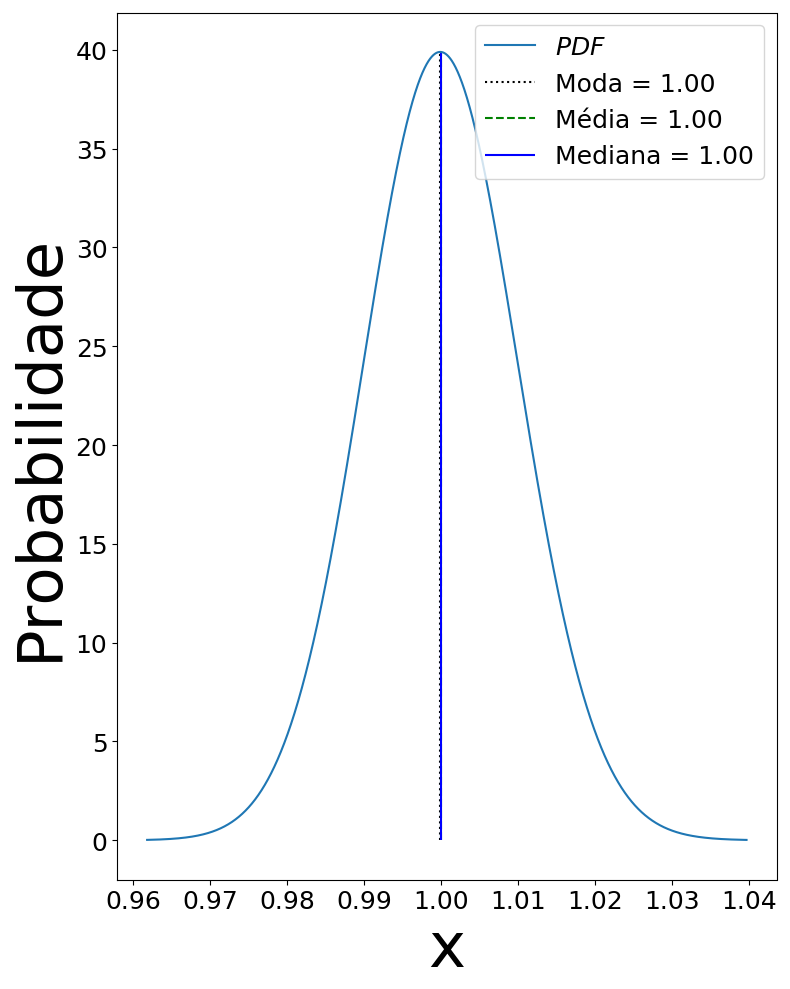
\includegraphics[width=\textwidth]{./figuras/log_sigma_001.png}
		\caption{}
		\label{fig:sig001}
	\end{subfigure}
	\hfill
	\begin{subfigure}[b]{0.3\textwidth}
		\centering 
		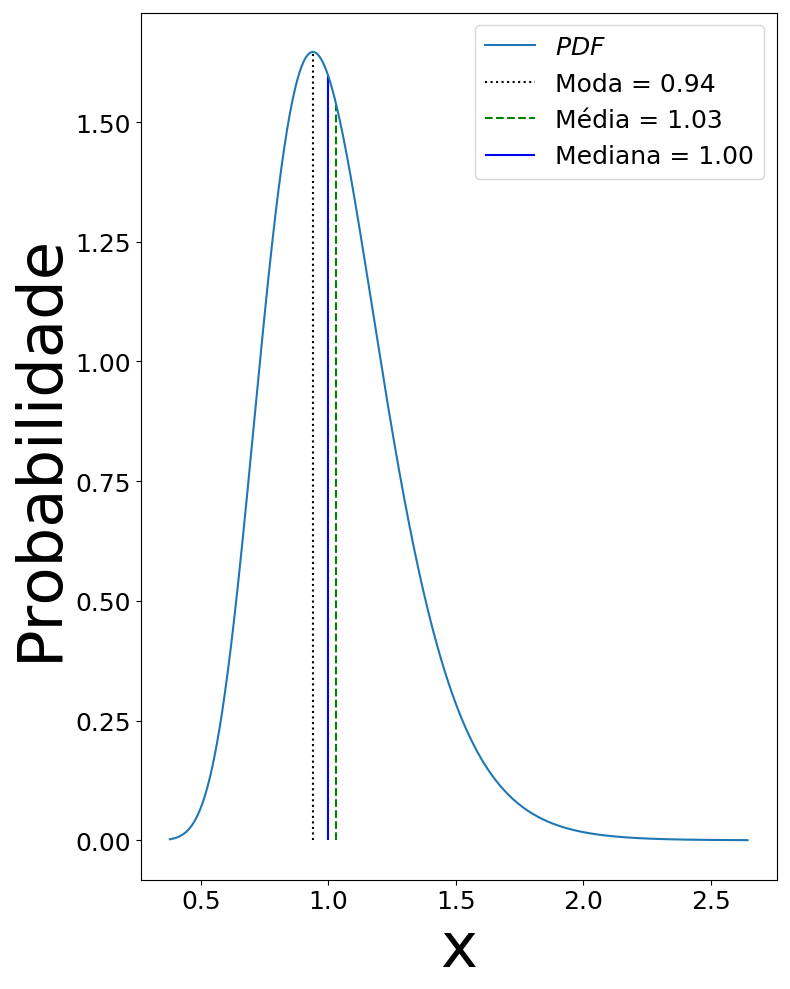
\includegraphics[width=\textwidth]{./figuras/log_sigma_025}
		\caption{}
		\label{fig:sig025}
	\end{subfigure}
	\hfill
	\begin{subfigure}[b]{0.3\textwidth}
		\centering 
		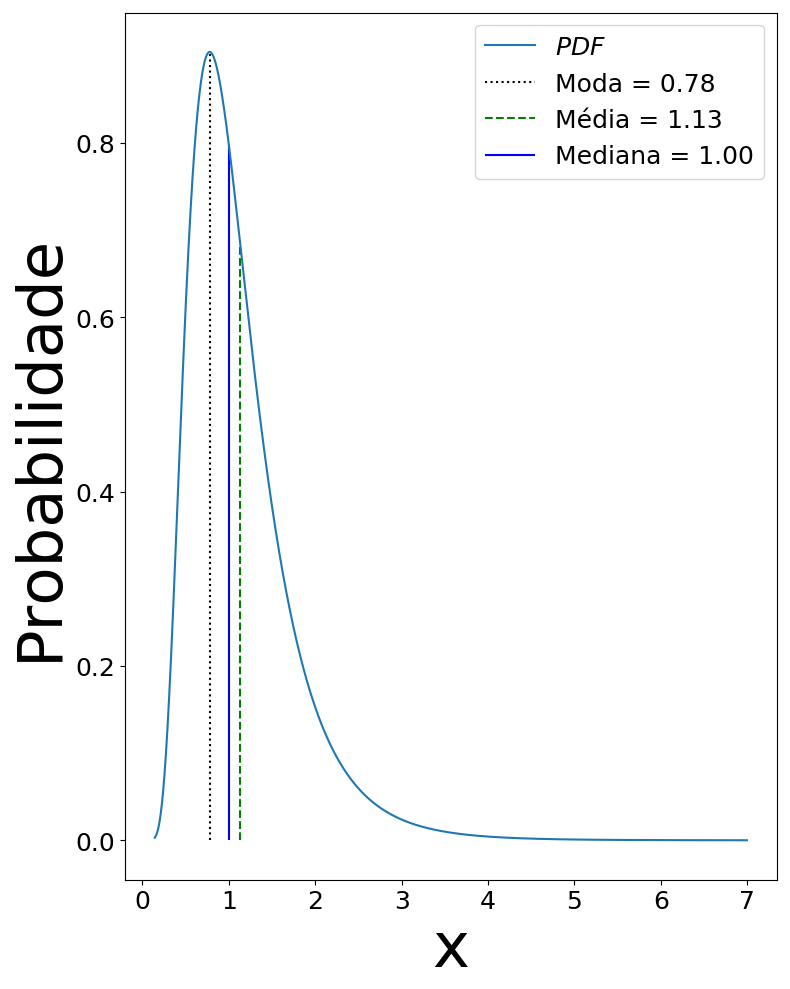
\includegraphics[width=\textwidth]{./figuras/log_sigma_05}
		\caption{}
		\label{fig:sig050}
	\end{subfigure}
	
	\begin{subfigure}[b]{0.3\textwidth}
		\centering 
		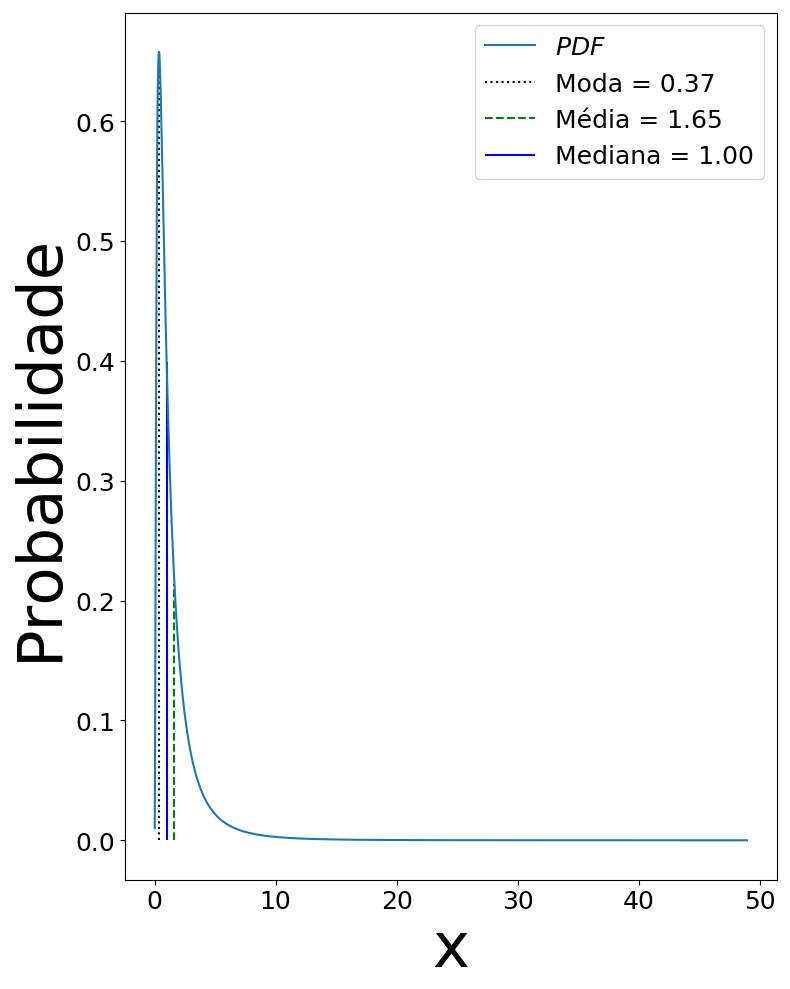
\includegraphics[width=\textwidth]{./figuras/log_sigma_1}
		\caption{}
		\label{fig:sig100}
	\end{subfigure}
	\hfill
	\begin{subfigure}[b]{0.3\textwidth}
		\centering 
		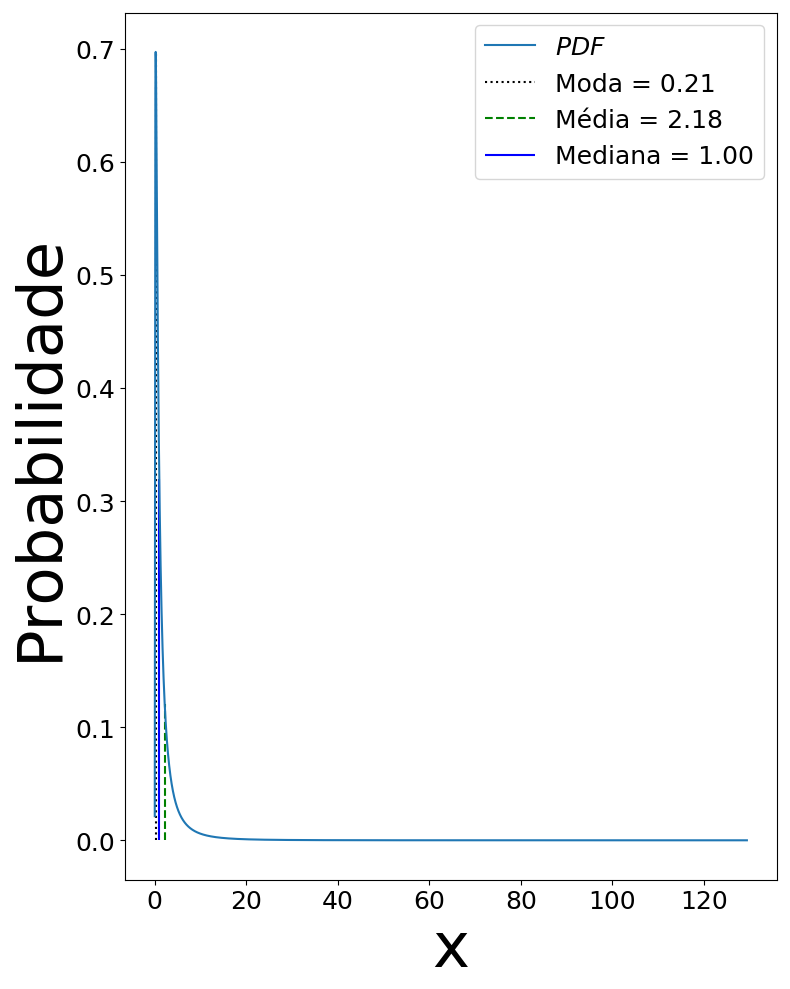
\includegraphics[width=\textwidth]{./figuras/log_sigma_125}
		\caption{}
		\label{fig:sig125}
	\end{subfigure}
	\hfill
	\begin{subfigure}[b]{0.3\textwidth}
		\centering 
		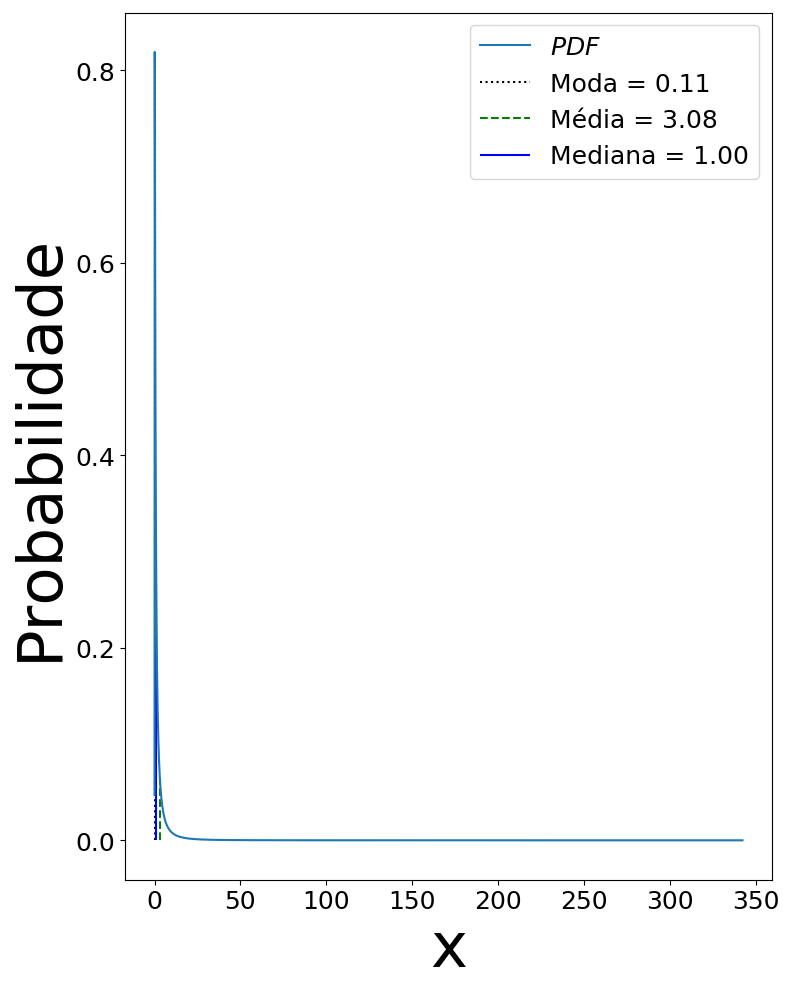
\includegraphics[width=\textwidth]{./figuras/log_sigma_15}
		\caption{}
		\label{fig:sig150}
	\end{subfigure}
	
	\caption{Ilustração das curvas Lognormais construidas com diferentes parâmetros: (a) possui $\sigma = 0.01$; (b) possui $\sigma = 0.25$; (c) possui $\sigma = 0.5$; (d) possui $\sigma = 1$; (e) possui $\sigma = 1.25$; e (f) possui $\sigma = 1.5$}
	\label{fig:Lognormal}
\end{figure}



\begin{figure}[H]
	\centering
	\begin{subfigure}[b]{0.27\textwidth}
		\centering 
		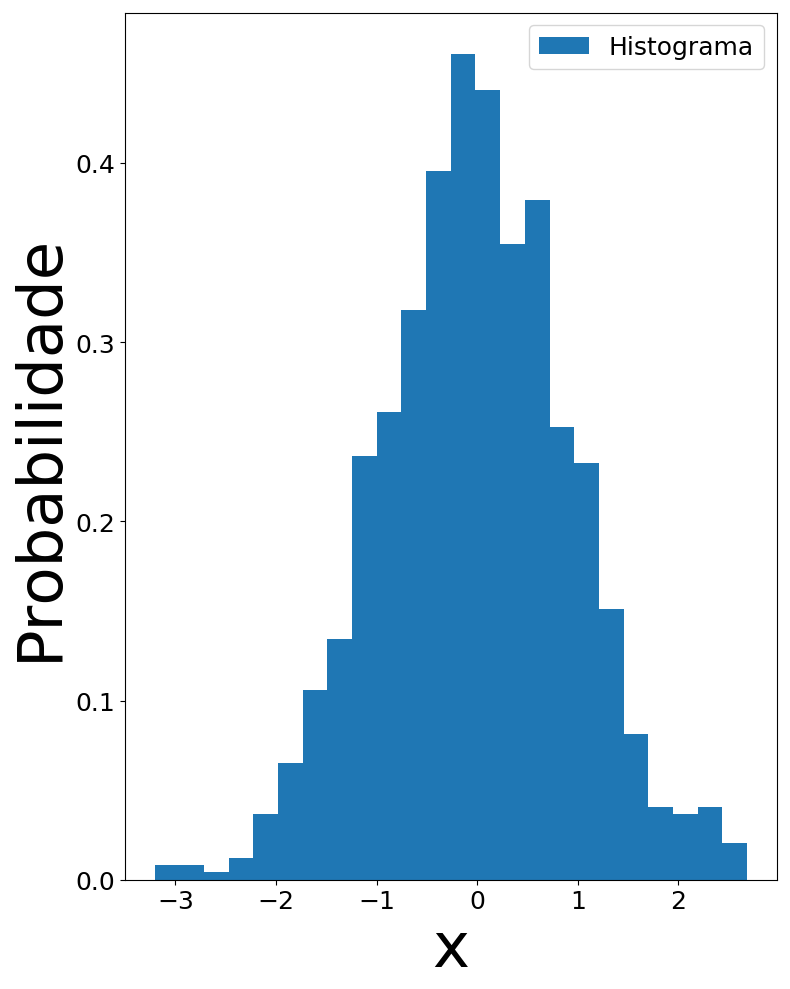
\includegraphics[width=\linewidth]{./figuras/datanormal_0}
		\caption{}
		\label{fig:randn}
	\end{subfigure}
	\hfill
	\begin{subfigure}[b]{0.27\textwidth}
		\centering 
		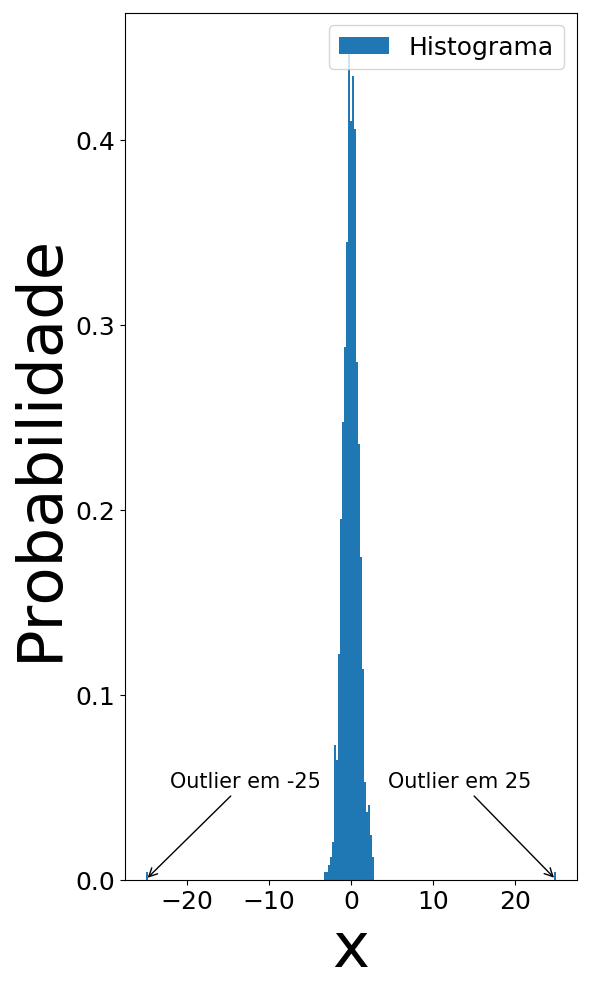
\includegraphics[width=\linewidth]{./figuras/datanormal_25}
		\caption{}
		\label{fig:randn_out}
	\end{subfigure}
	\hfill
	\begin{subfigure}[b]{0.27\textwidth}
		\centering 
		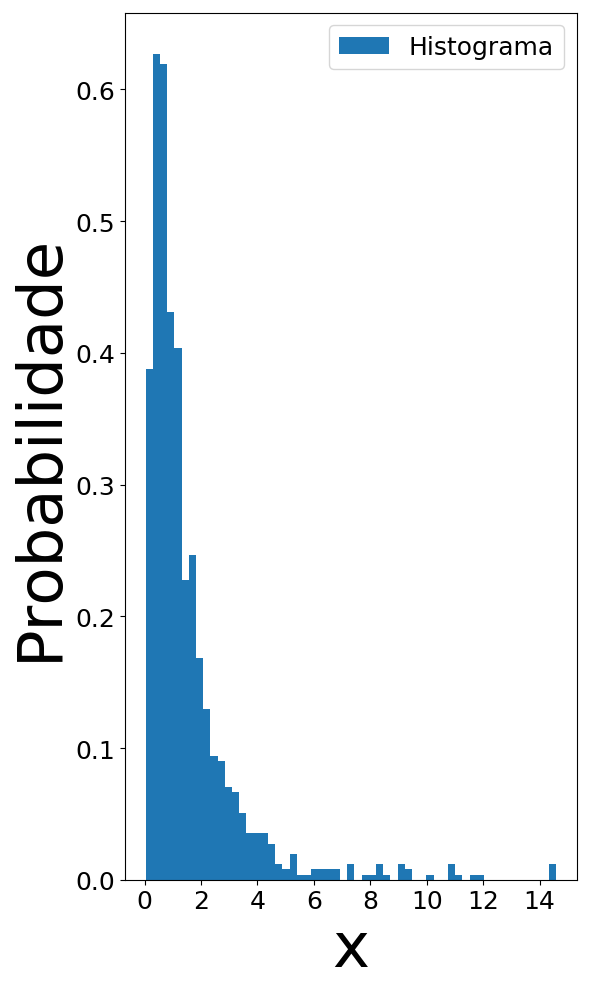
\includegraphics[width=\linewidth]{./figuras/datalognormal_0}
		\caption{}
		\label{fig:randlog}
	\end{subfigure}
	
	\caption{Histograma dos dados gerados sendo eles: (a) Gaussiana com $\mu = 0$ e $\sigma$ = 1; (b) Gaussiana com $\mu = 0$, $\sigma = 1$ e \textit{outlier} em $\pm 25$; (c) Lognormal com $\mu = 0$ e $\sigma = 0.5$.}
	\label{fig:data}
\end{figure}

\section{Algoritmo}
{\color{red} Não entendi muito bem o que é pra colocar aqui, seria apenas o algoritmo da discretização? pq este meio que já foi explicado no cap 2 né, quando eu explico como cada método funciona. Talvez seja mais interessante botar isso aqui lá pro final, explicando como os erros foram calculados, o que achas?}

\section{Ambiente de Análise}
Aqui iremos testar todas os métodos apresentados até o momento para diferentes distribuições variando o número de estimação para $ N = 15 $ e $ N = 25 $
\subsection{Gaussiana}

Utilizando como base a Figura~\ref{fig:Gaussiana}

\subsubsection{\textit{Linspace}}

\begin{figure}[H]
	\centering
	\begin{subfigure}[b]{0.45\textwidth}
		\centering 
		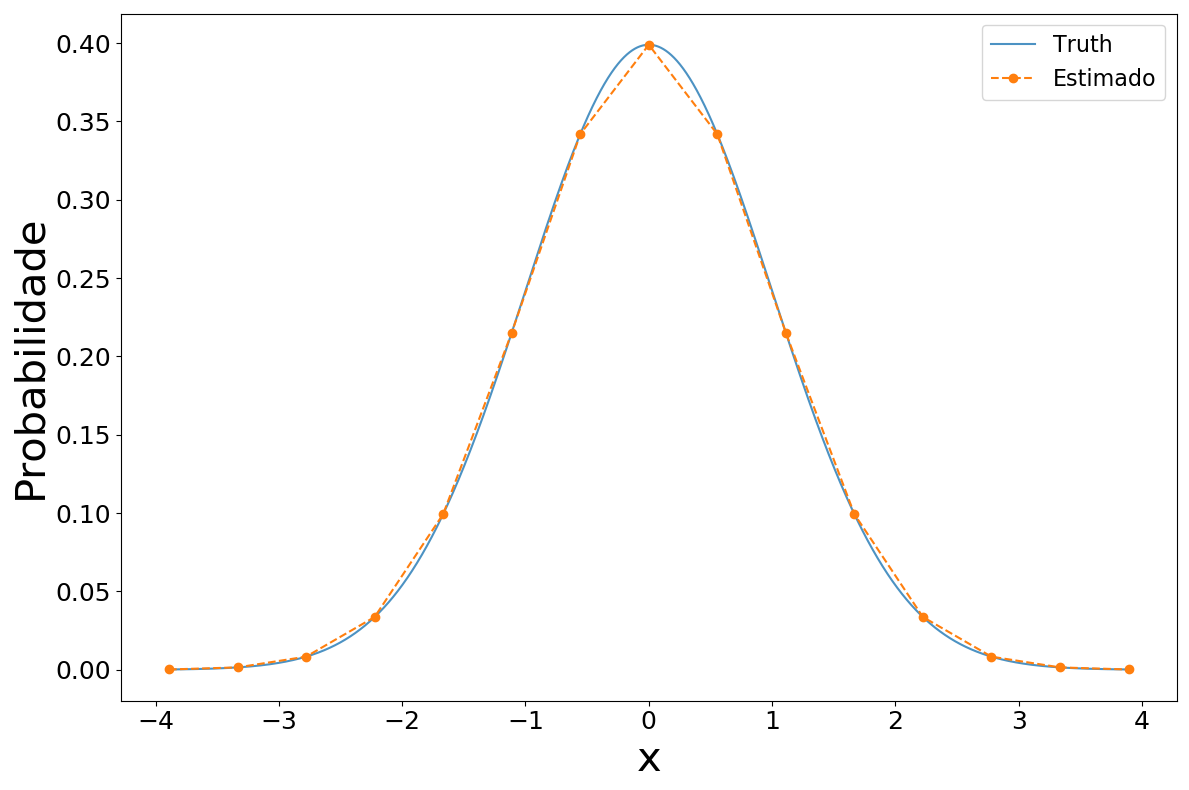
\includegraphics[width=\linewidth]{./figuras/normal_15}
		\caption{}
		\label{fig:norm15}
	\end{subfigure}
	\hfill
	\begin{subfigure}[b]{0.45\textwidth}
		\centering 
		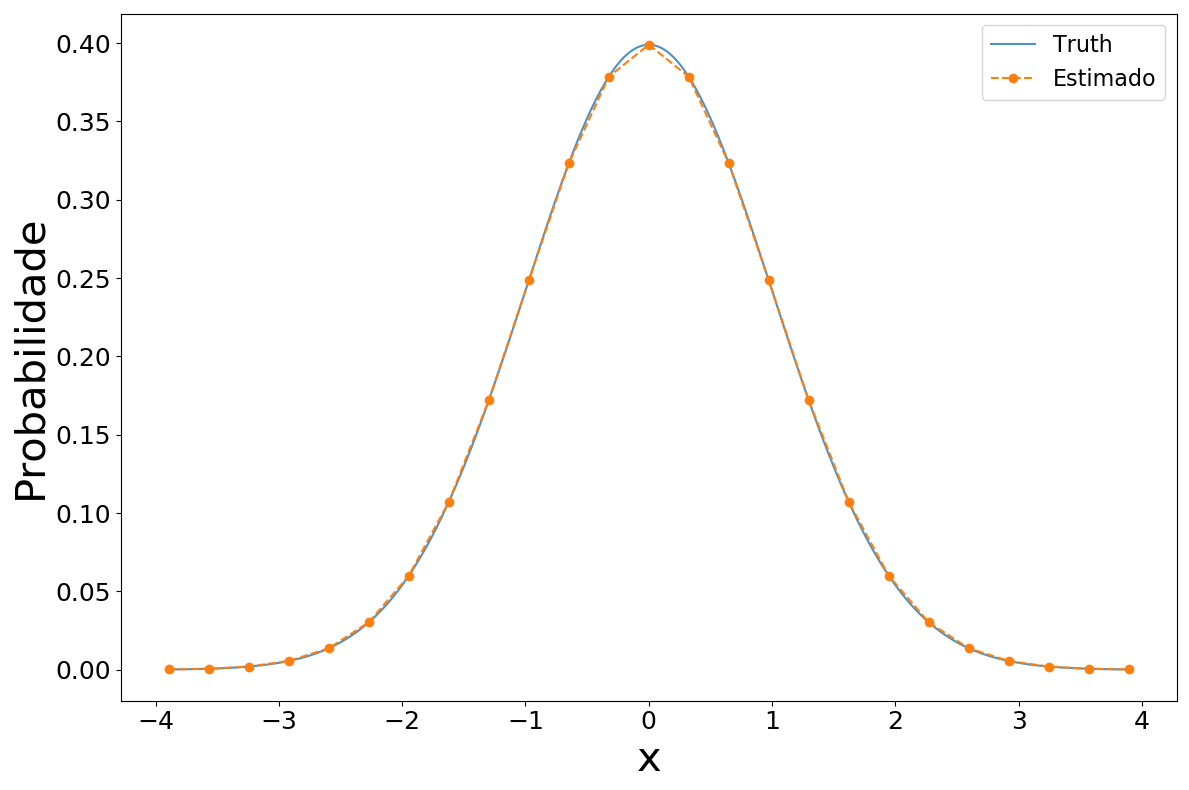
\includegraphics[width=\linewidth]{./figuras/normal_25}
		\caption{}
		\label{fig:norm25}
	\end{subfigure}
	
	\caption{Discretização da distribuição Normal utilizando-se o método \textit{Linspace}: (a) Discretização utilizando-se 15 pontos de estimação; (b) Discretização utilizando-se 25 pontos de estimação.}
	\label{fig:normlin}
\end{figure}

Podemos perceber que para este método, mesmo com quinze pontos de estimação, o método conseguiu descrever bem a curva, acentuando o erro nas regiões de alta probabilidade.

\subsubsection{\textit{CDFm}}


\begin{figure}[H]
	\centering
	\begin{subfigure}[b]{0.45\textwidth}
		\centering 
		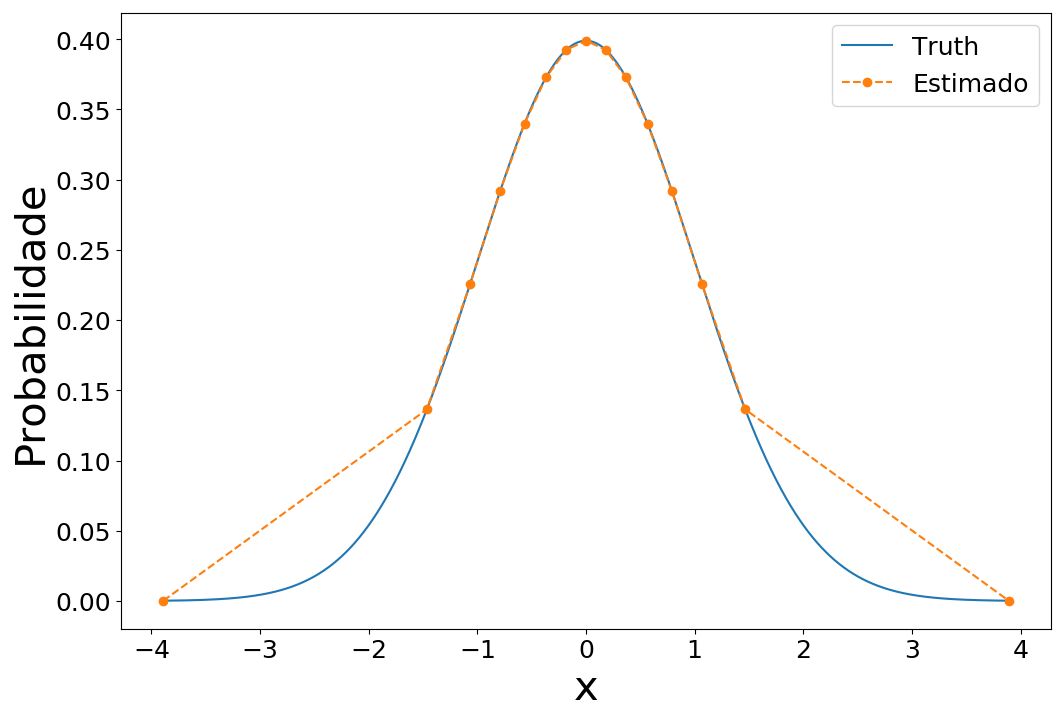
\includegraphics[width=\linewidth]{./figuras/CDFm_normal_15}
		\caption{}
		\label{fig:cdfnorm15}
	\end{subfigure}
	\hfill
	\begin{subfigure}[b]{0.45\textwidth}
		\centering 
		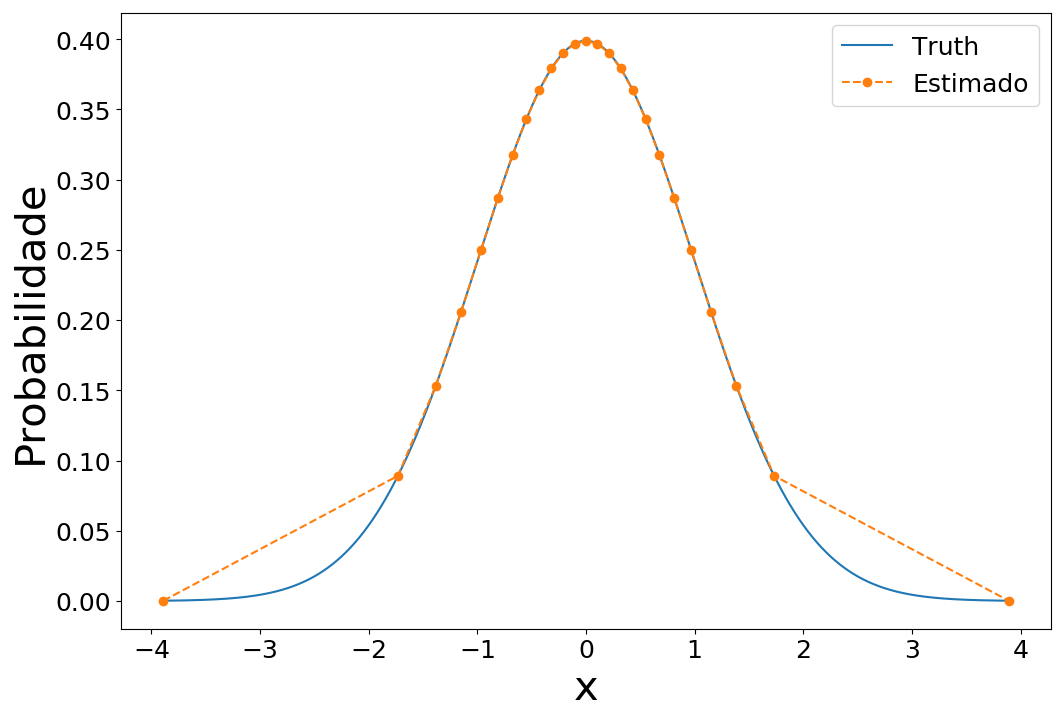
\includegraphics[width=\linewidth]{./figuras/CDFm_normal_25}
		\caption{}
		\label{fig:cdfnorm25}
	\end{subfigure}
	
	\caption{Discretização da distribuição Normal utilizando-se o método \textit{CDFm}: (a) Discretização utilizando-se 15 pontos de estimação; (b) Discretização utilizando-se 25 pontos de estimação.}
	\label{fig:cdfnorm}
\end{figure}

Vemos que a região de alta probabilidade é representada com um menor erro do que no método \textit{Linspace} mas, em contrapartida, a região de baixa probabilidade necessitaria de um número muito maior de pontos para possuir o mesmo erro do método anterior.

\subsubsection{\textit{PDFm}}

\begin{figure}[H]
	\centering
	\begin{subfigure}[b]{0.45\textwidth}
		\centering 
		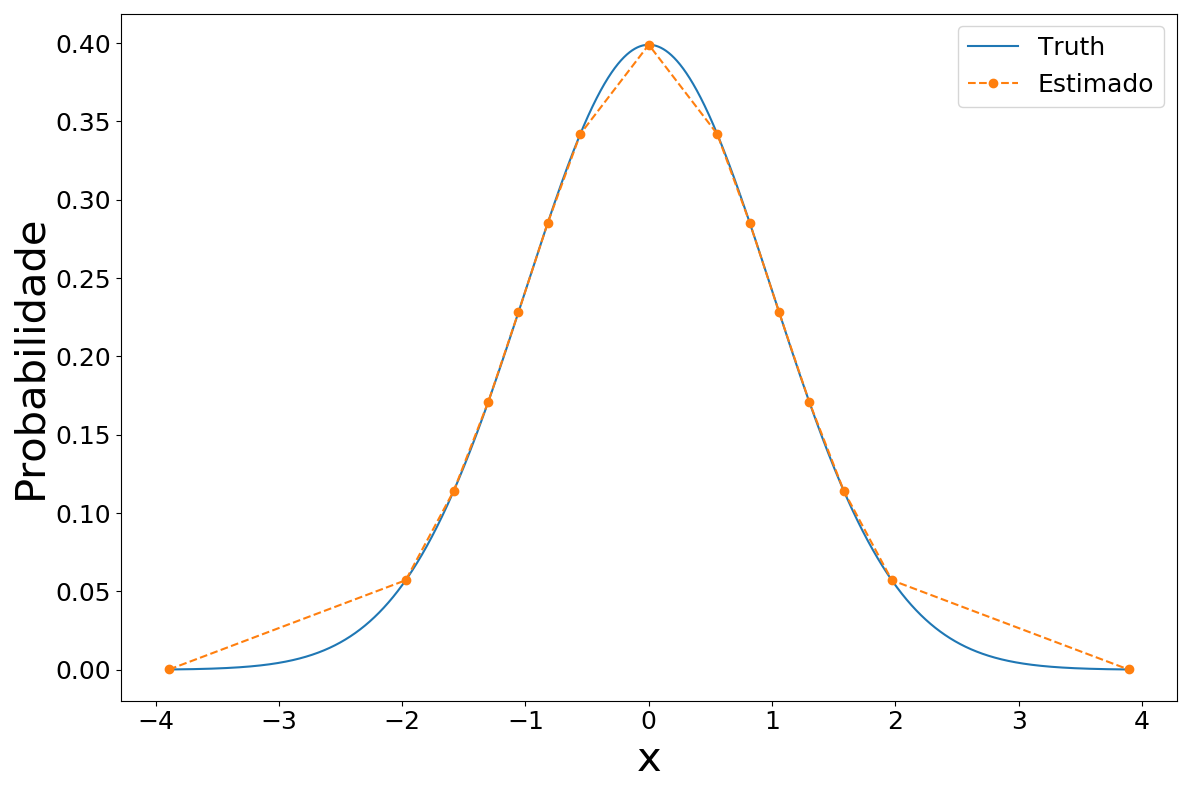
\includegraphics[width=\linewidth]{./figuras/PDFm_normal_15}
		\caption{}
		\label{fig:pdfnorm15}
	\end{subfigure}
	\hfill
	\begin{subfigure}[b]{0.45\textwidth}
		\centering 
		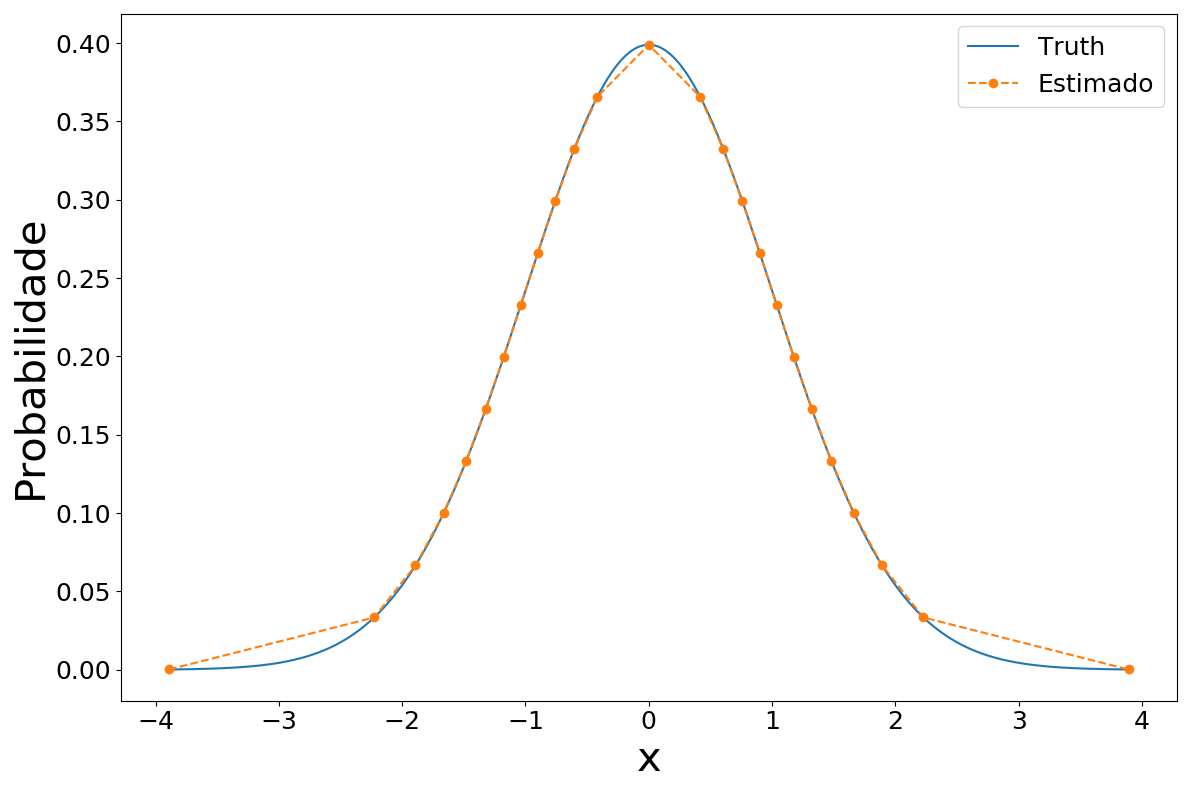
\includegraphics[width=\linewidth]{./figuras/PDFm_normal_25}
		\caption{}
		\label{fig:pdfnorm25}
	\end{subfigure}
	
	\caption{Discretização da distribuição Normal utilizando-se o método \textit{PDFm}: (a) Discretização utilizando-se 15 pontos de estimação; (b) Discretização utilizando-se 25 pontos de estimação.}
	\label{fig:pdfmnorm}
\end{figure}

Para a distribuição Normal, este método apresenta um maior erro na região de alta probabilidade do que o método \ac{CDFm} mas nas regiões de baixa probabilidade o erro de estimação é menor do que o visto anteriormente, fazendo assim uma combinação dos métodos \textit{Linspace} e \textit{CDFm}.
 
\subsubsection{\textit{iPDF1}}

\begin{figure}[H]
	\centering
	\begin{subfigure}[b]{0.45\textwidth}
		\centering 
		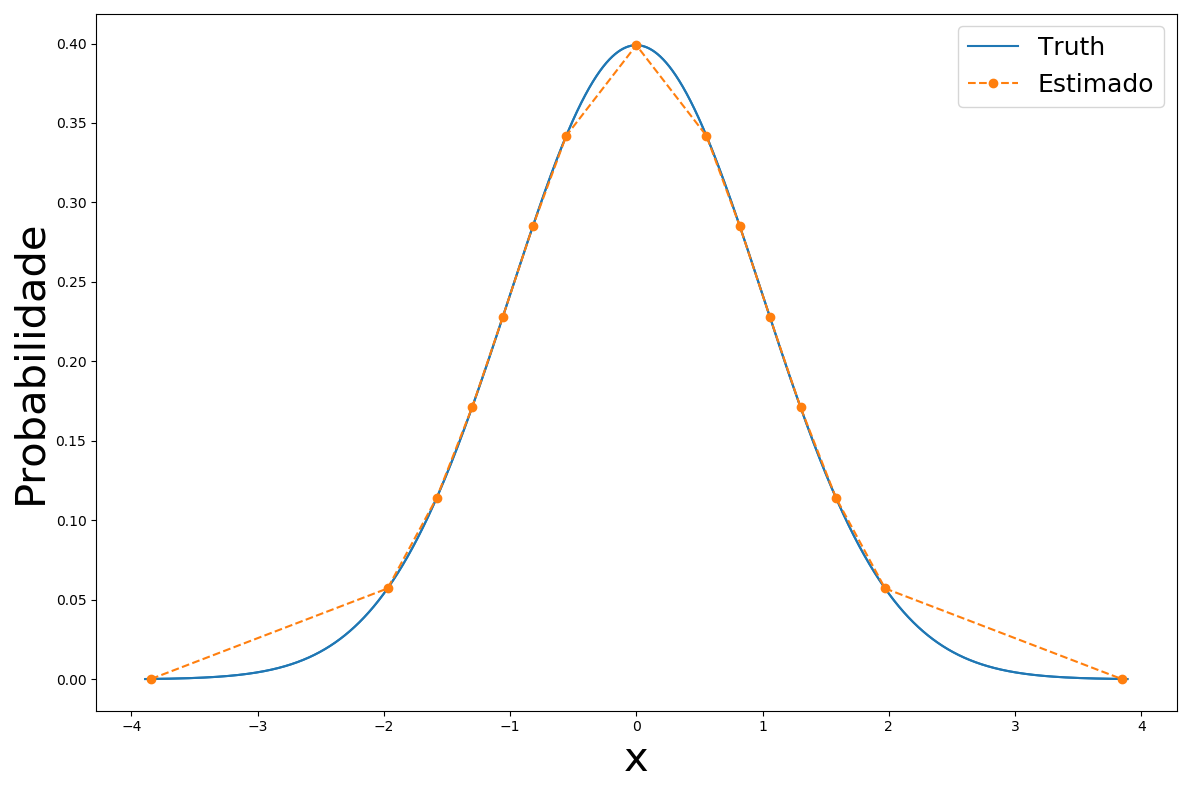
\includegraphics[width=\linewidth]{./figuras/iPDF1_normal_15}
		\caption{}
		\label{fig:ipdfnorm15}
	\end{subfigure}
	\hfill
	\begin{subfigure}[b]{0.45\textwidth}
		\centering 
		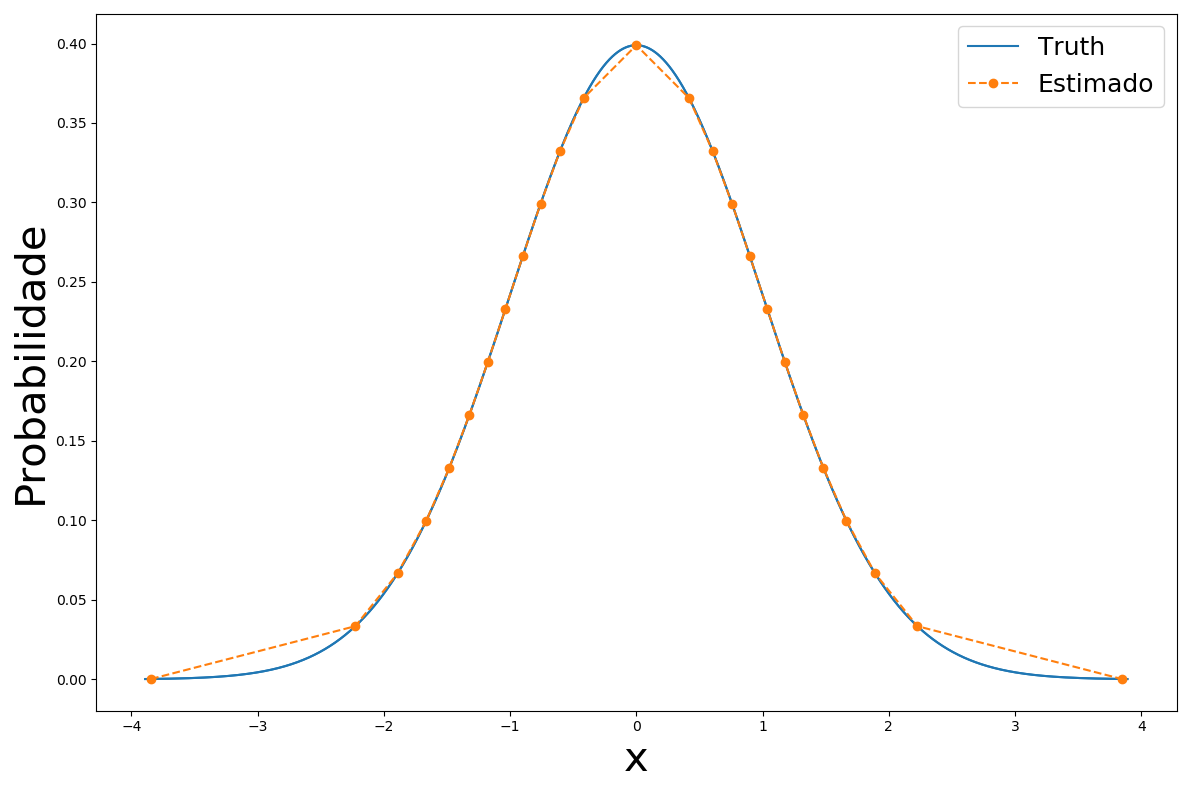
\includegraphics[width=\linewidth]{./figuras/iPDF1_normal_25}
		\caption{}
		\label{fig:ipdfnorm25}
	\end{subfigure}
	
	\caption{Discretização da distribuição Normal utilizando-se o método \textit{iPDF1}: (a) Discretização utilizando-se 15 pontos de estimação; (b) Discretização utilizando-se 25 pontos de estimação.}
	\label{fig:ipdfmnorm}
\end{figure}



\subsubsection{\textit{iPDF2}}

\begin{figure}[H]
	\centering
	\begin{subfigure}[b]{0.45\textwidth}
		\centering 
		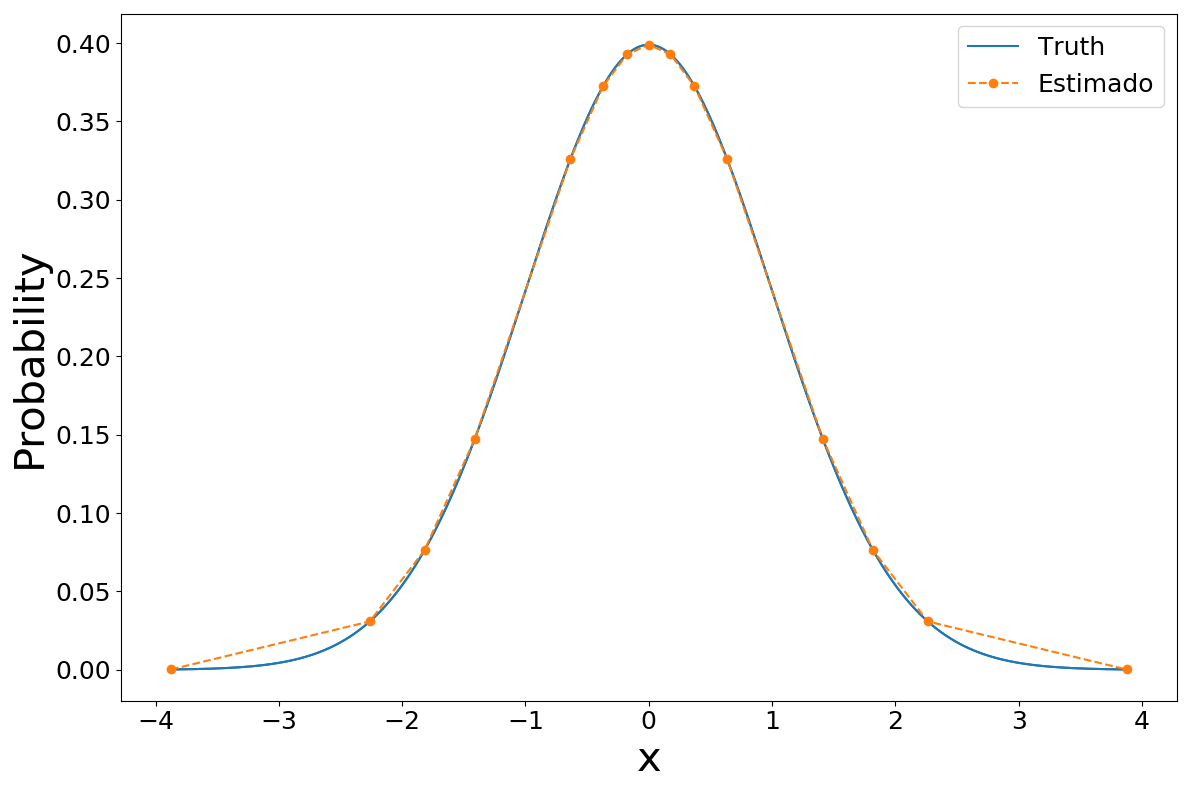
\includegraphics[width=\linewidth]{./figuras/iPDF2_normal_15}
		\caption{}
		\label{fig:ipdf2norm15}
	\end{subfigure}
	\hfill
	\begin{subfigure}[b]{0.45\textwidth}
		\centering 
		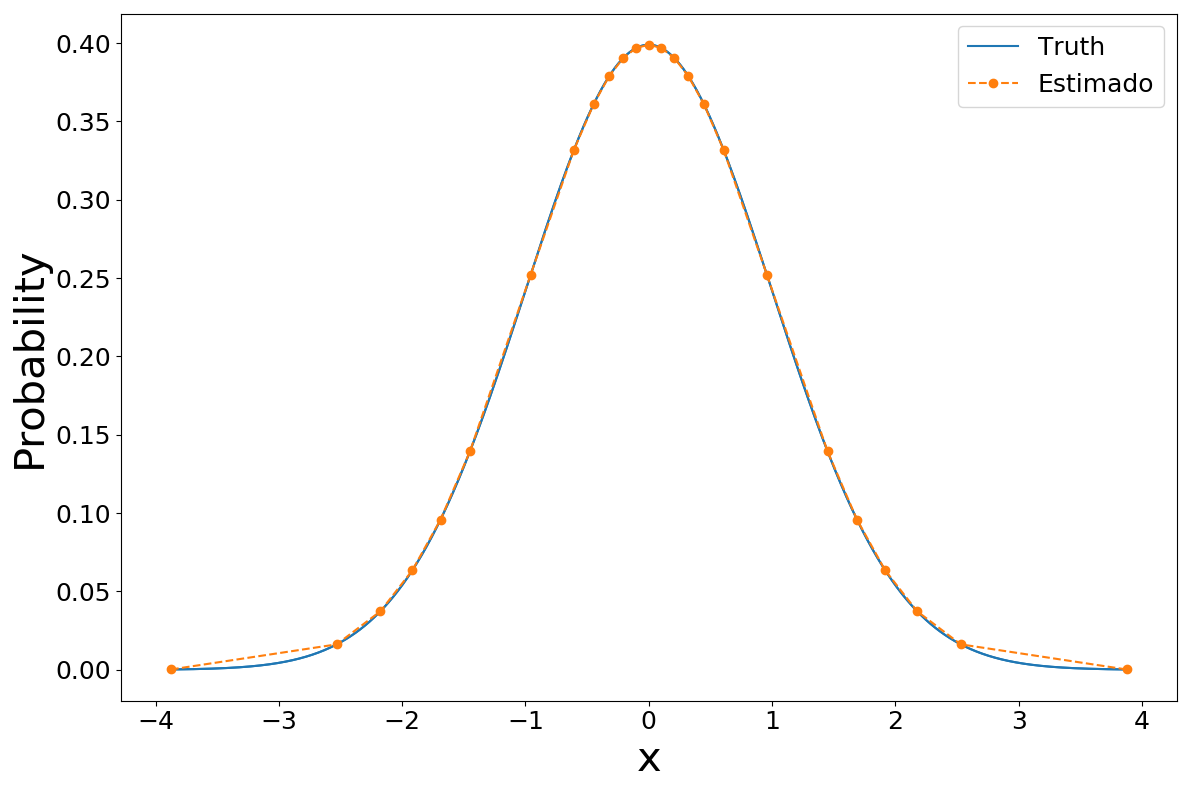
\includegraphics[width=\linewidth]{./figuras/iPDF2_normal_25}
		\caption{}
		\label{fig:ipdf2norm25}
	\end{subfigure}
	
	\caption{Discretização da distribuição Normal utilizando-se o método \textit{iPDF2}: (a) Discretização utilizando-se 15 pontos de estimação; (b) Discretização utilizando-se 25 pontos de estimação.}
	\label{fig:ipdf2norm}
\end{figure}

\subsection{Lognormal}

\subsubsection{\textit{Linspace}}
\subsubsection{\textit{CDFm}}
\subsubsection{\textit{PDFm}}
\subsubsection{\textit{iPDF1}}
\subsubsection{\textit{iPDF2}}
\subsection{Dataset}

\subsubsection{\textit{Linspace}}
\subsubsection{\textit{CDFm}}
\subsubsection{\textit{PDFm}}
\subsubsection{\textit{iPDF1}}
\subsubsection{\textit{iPDF2}}

\subsection{\textit{Linspace}}
O método \textit{Linspace} é caracterizado por amostrar de maneira uniforme a variável aleatória, representada pelo eixo das abscissas de uma \ac{PDF} dada. Após, o eixo horizontal terá \textit{N} pontos igualmente espaçados entre dois valores predefinidos que definem os parâmetros de início e término da distribuição. Este método é o mais utilizado na literatura devido a sua simplicidade. A Figura~\ref{fig:linspace_curve} ilustra o método \textit{Linspace} para a distribuição Normal e a Figura~\ref{fig:Lognormal_lin} ilustra o mesmo método para uma distribuição Lognormal com diferentes desvios padrões, limitando o eixo horizontal à uma área de probabilidade de $99.99\%$. A Figura~\ref{fig:datalin} mostra as distribuições geradas, conforme é mostrado na Figura~\ref{fig:data}, discretizadas utilizando este método.

\begin{figure}[H]
	\centering
	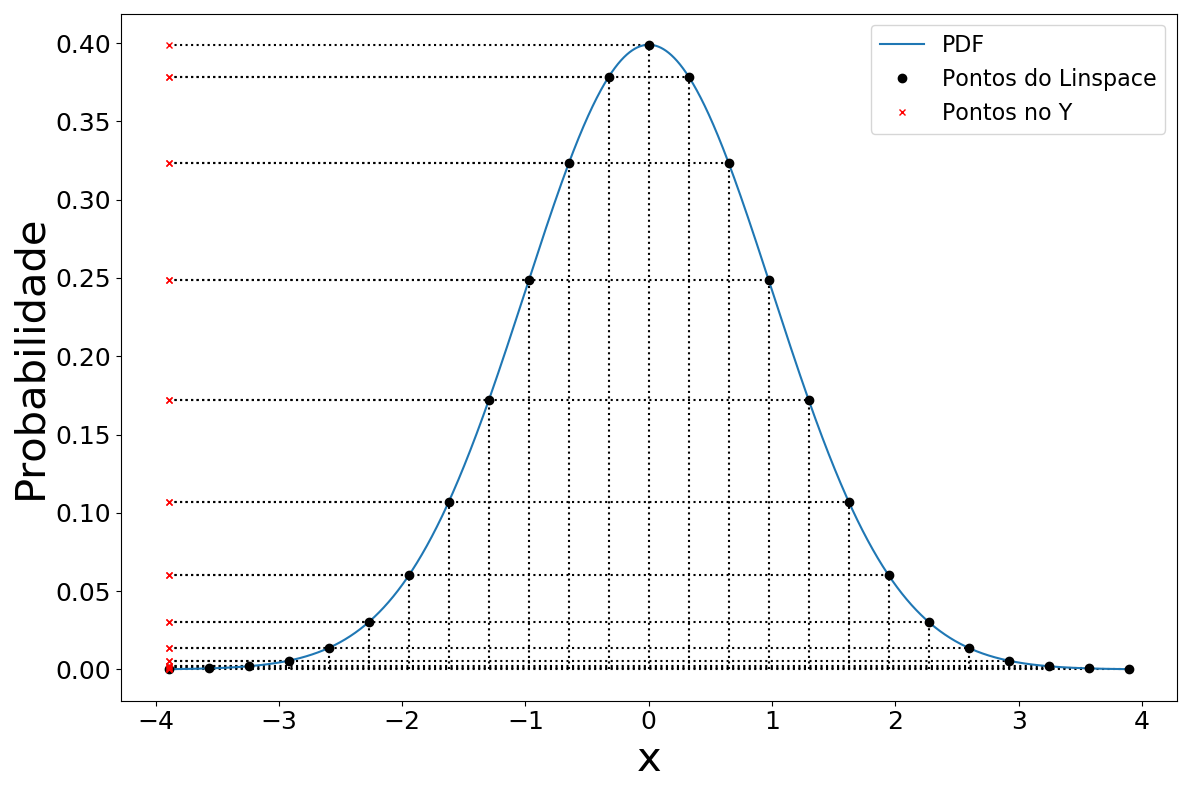
\includegraphics[width=0.7\linewidth]{./figuras/normal_1}
	\caption{Ilustração do método Linspace aplicado à uma distribuição normal.}
	\label{fig:linspace_curve}
\end{figure}

\begin{figure}[H]
	\centering
	\begin{subfigure}[b]{0.3\textwidth}
		\centering 
		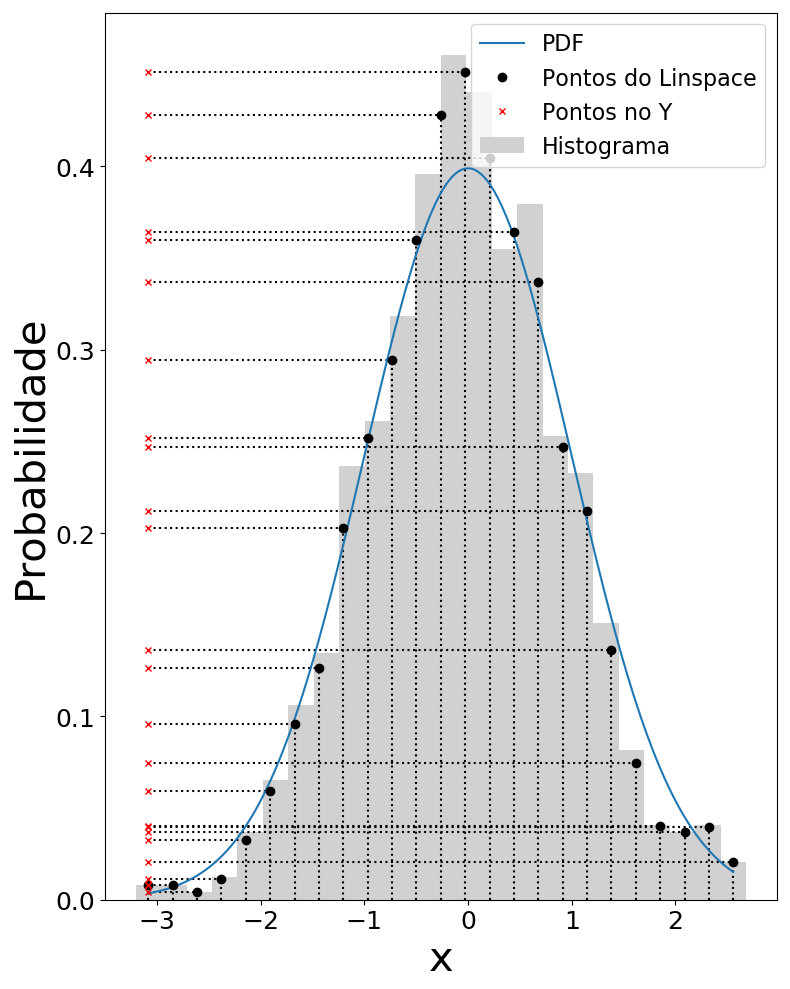
\includegraphics[width=\linewidth]{./figuras/normal_1_0}
		\caption{}
		\label{fig:randnlin}
	\end{subfigure}
	\hfill
	\begin{subfigure}[b]{0.3\textwidth}
		\centering 
		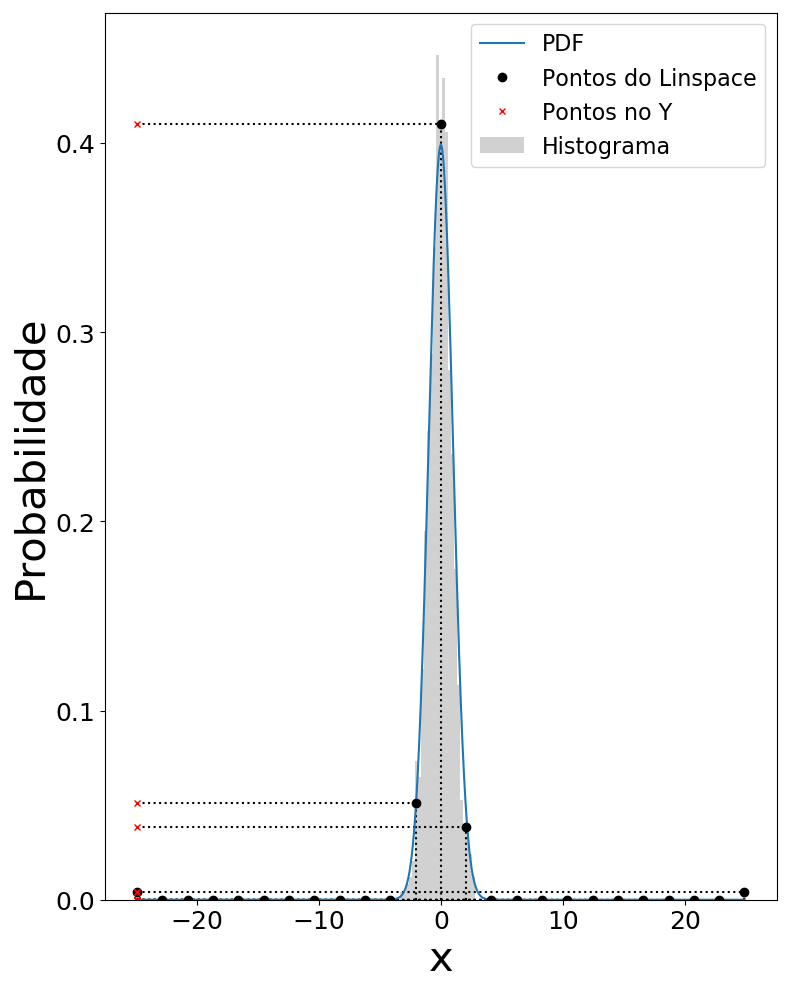
\includegraphics[width=\linewidth]{./figuras/normal_1_25}
		\caption{}
		\label{fig:randn_outlin}
	\end{subfigure}
	\hfill
	\begin{subfigure}[b]{0.3\textwidth}
		\centering 
		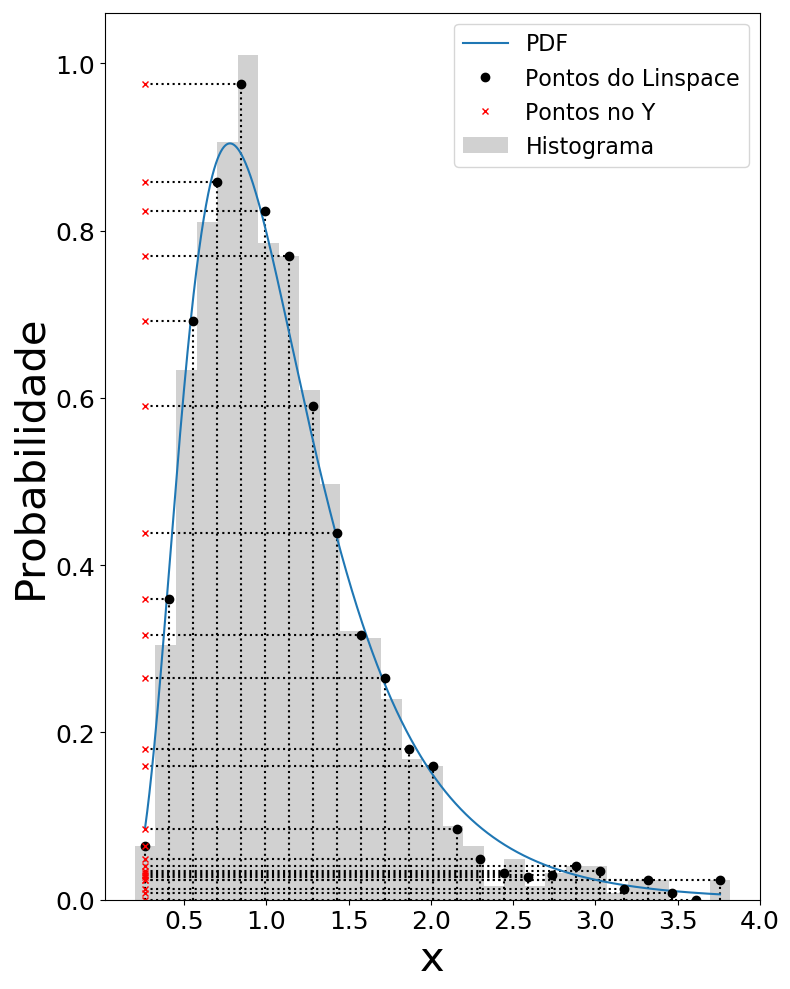
\includegraphics[width=\linewidth]{./figuras/lognormal_05_0}
		\caption{}
		\label{fig:randloglin}
	\end{subfigure}
	
	\caption{Histograma dos dados gerados utilizando a discretização pelo método \textit{Linspace} sendo eles: (a) Gaussiana com $\mu = 0$ e $\sigma$ = 1; (b) Gaussiana com $\mu = 0$, $\sigma = 1$ e \textit{outlier} em $\pm 25$; (c) Lognormal com $\mu = 0$ e $\sigma = 0.5$.}
	\label{fig:datalin}
\end{figure}


\begin{figure}[H]
	\centering
	\begin{subfigure}[b]{0.3\textwidth}
		\centering 
		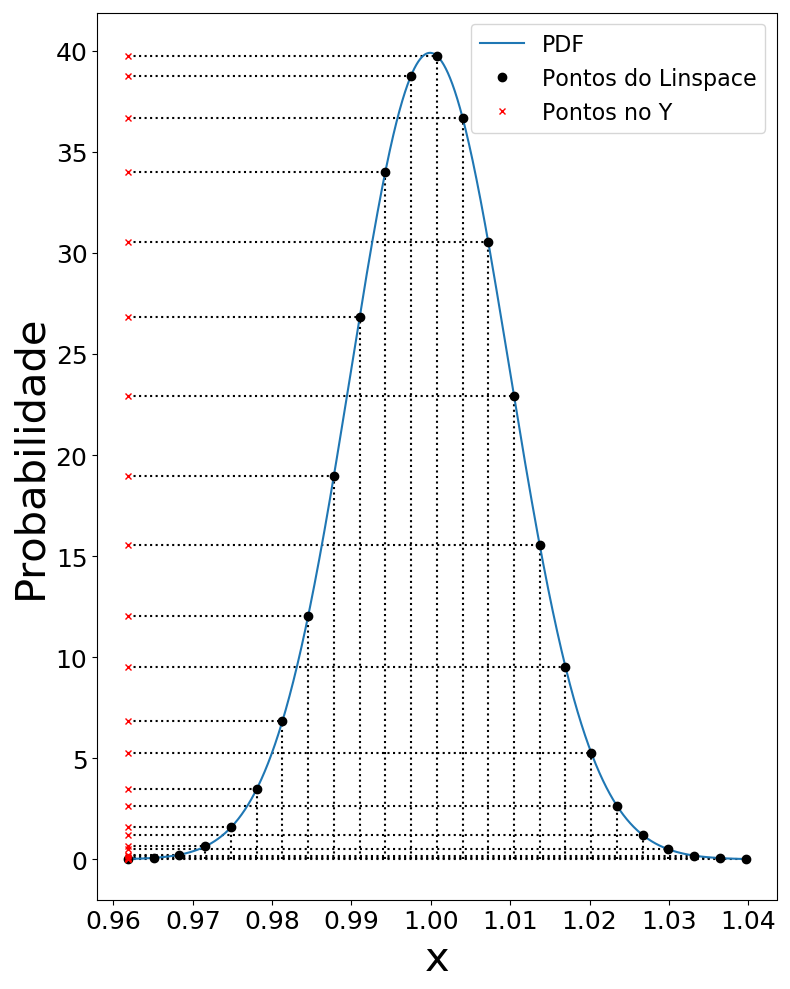
\includegraphics[width=\textwidth]{./figuras/lognormal_001.png}
		\caption{}
		\label{fig:lin001}
	\end{subfigure}
	\hfill
	\begin{subfigure}[b]{0.3\textwidth}
		\centering 
		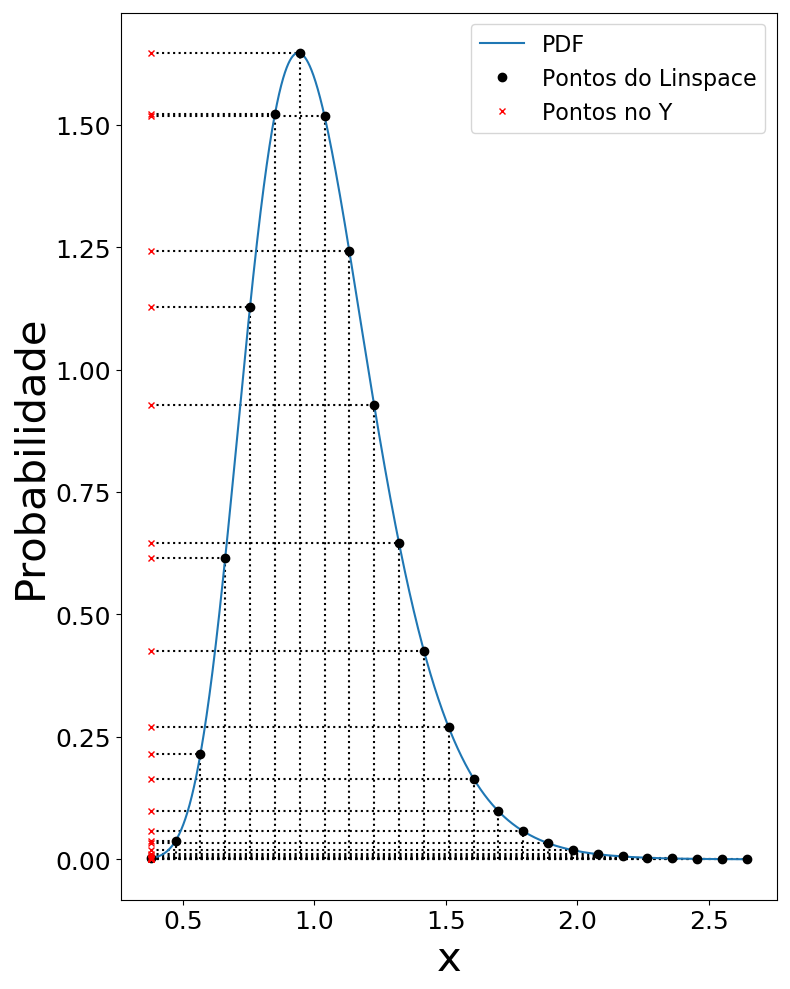
\includegraphics[width=\textwidth]{./figuras/lognormal_025}
		\caption{}
		\label{fig:lin025}
	\end{subfigure}
	\hfill
	\begin{subfigure}[b]{0.3\textwidth}
		\centering 
		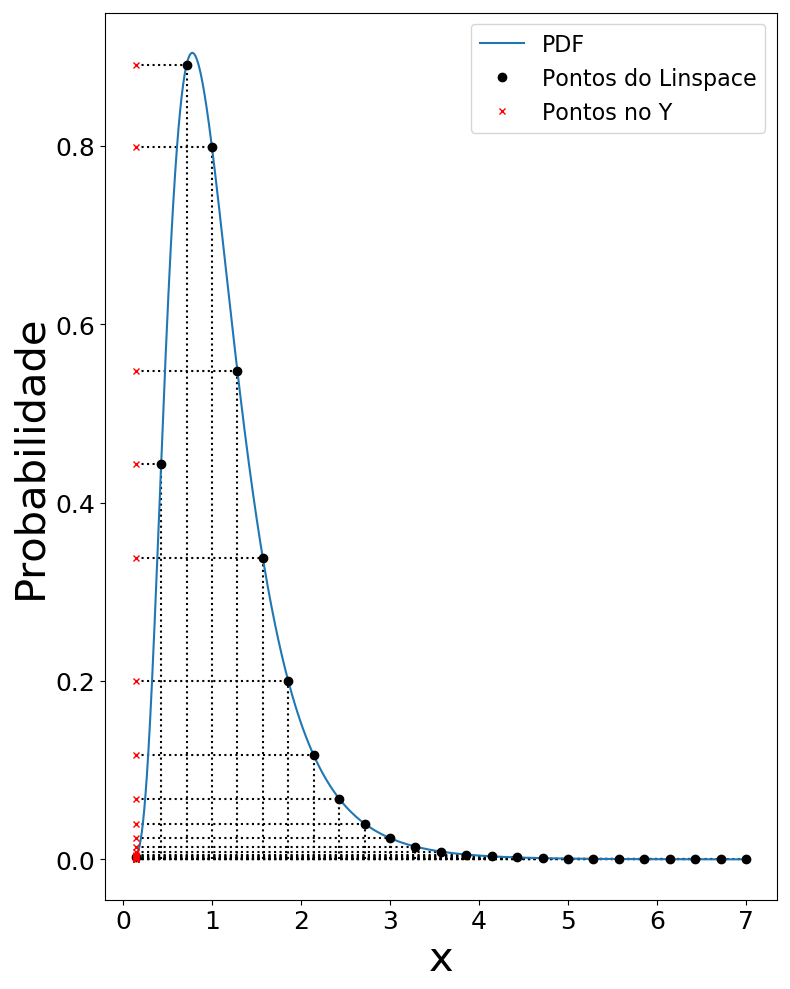
\includegraphics[width=\textwidth]{./figuras/lognormal_05}
		\caption{}
		\label{fig:lin050}
	\end{subfigure}
	
	\begin{subfigure}[b]{0.3\textwidth}
		\centering 
		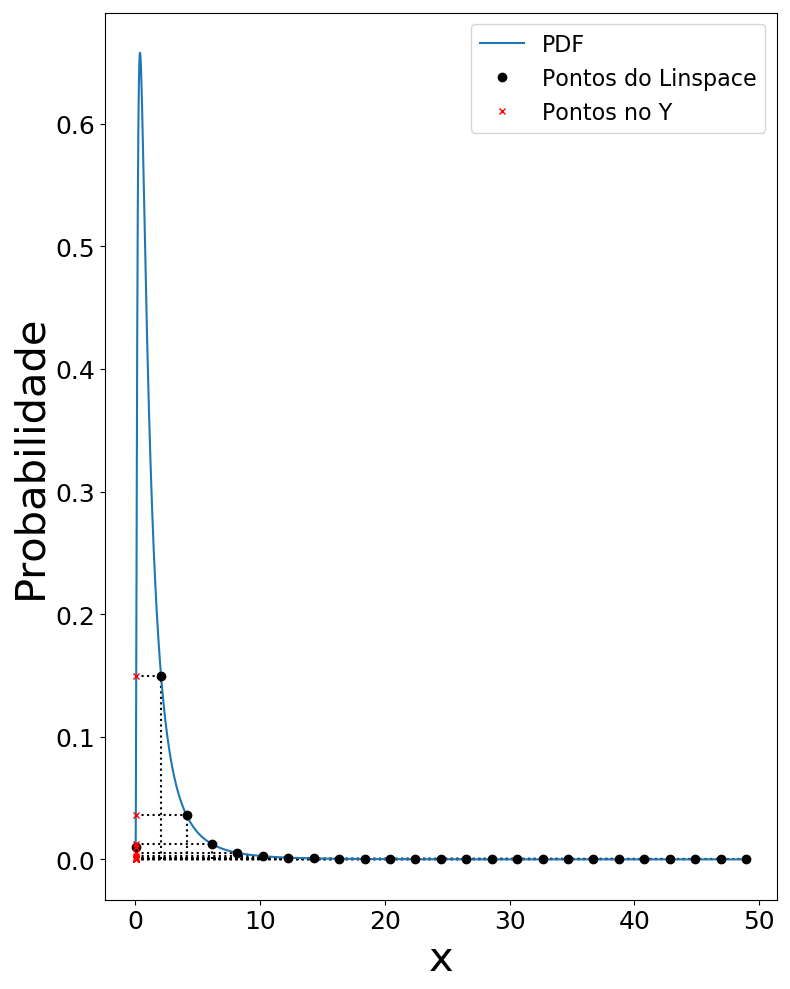
\includegraphics[width=\textwidth]{./figuras/lognormal_1}
		\caption{}
		\label{fig:lin100}
	\end{subfigure}
	\hfill
	\begin{subfigure}[b]{0.3\textwidth}
		\centering 
		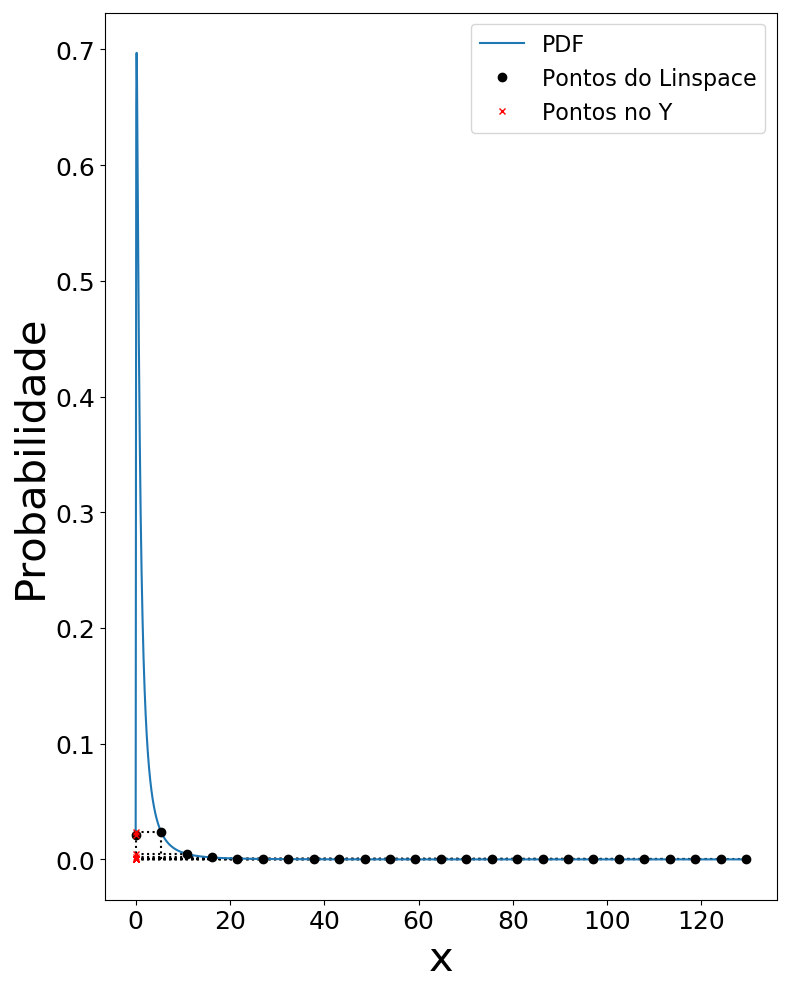
\includegraphics[width=\textwidth]{./figuras/lognormal_125}
		\caption{}
		\label{fig:lin125}
	\end{subfigure}
	\hfill
	\begin{subfigure}[b]{0.3\textwidth}
		\centering 
		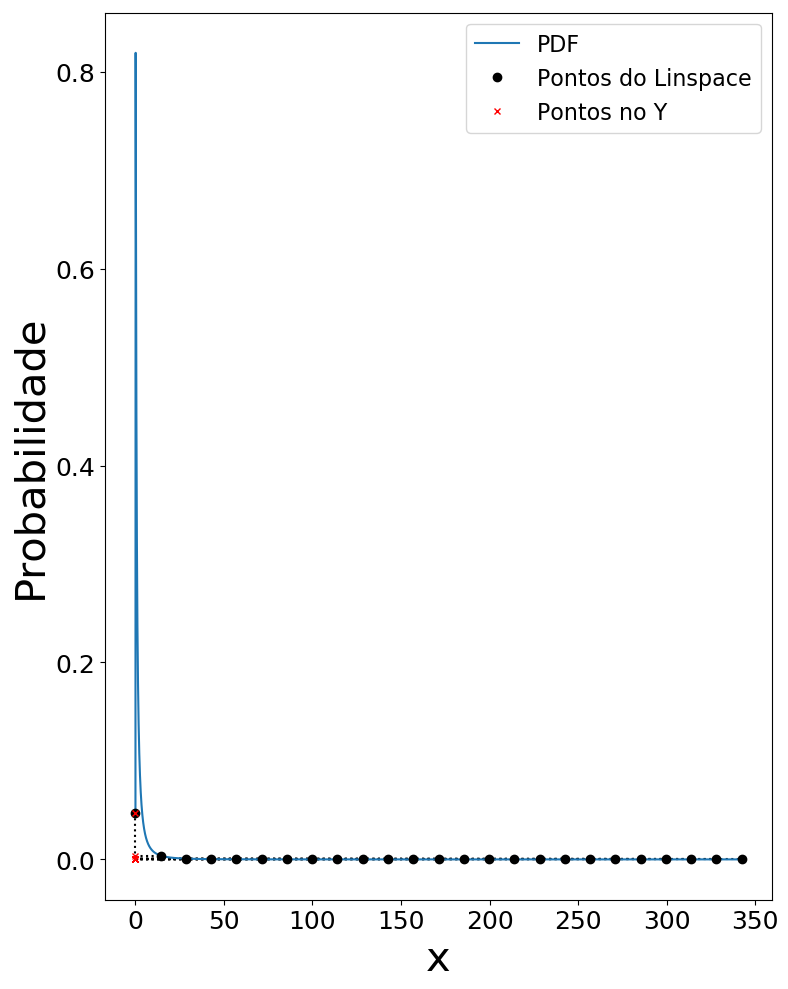
\includegraphics[width=\textwidth]{./figuras/lognormal_15}
		\caption{}
		\label{fig:lin150}
	\end{subfigure}
\caption{Ilustração do método Linspace aplicado à uma distribuição lognormal em que: (a) possui $\sigma = 0.01$; (b) possui $\sigma = 0.25$; (c) possui $\sigma = 0.5$; (d) possui $\sigma = 1$; (e) possui $\sigma = 1.25$; e (f) possui $\sigma = 1.5$}
\label{fig:Lognormal_lin}
\end{figure}


É possível perceber que este método atende de forma satisfatória distribuições que não possuem derivadas muito altas como é ilustrado na figura \ref{fig:linspace_curve} e nas figuras \ref{fig:lin001} à \ref{fig:lin050}, embora nas Figuras \ref{fig:randnlin} e \ref{fig:randloglin} há um erro de estimação por devida à quantidade de eventos simulados. Nas figuras \ref{fig:lin100} à \ref{fig:lin150} e \ref{fig:randn_outlin} o método em questão já não consegue descrever a curva, colocando um número insuficientes de pontos na região de alta probabilidade e um número maior de pontos na região de alta probabilidade.

\subsection{\textit{CDFm}}
O método denominado nesse trabalho de \ac{CDFm} representa a discretização baseada na \ac{CDF}. Para este método, a discretização baseada no espaçamento uniforme é aplicada ao eixo vertical e então os relativos valores horizontais são encontrados refletindo todos os valores, como mostra a Figura~\ref{fig:CDFm_curve} para a distribuição Normal, a Figura~\ref{fig:Lognormal_cdf} para a distribuição Lognormal e a Figura~XXXXX para o \textit{dataset}. Note que, quanto maior a probabilidade da \ac{PDF}, maior o número de pontos na sua região e que os \textit{outliers} não fazem mais tanto efeito, como é o caso do \textit{Linspace}.

\color{red} COLOCAR GRÁFICO 2X3 \color{black}

\begin{figure}[H]
	\centering
	\begin{subfigure}[b]{0.49\textwidth}
		\centering 
		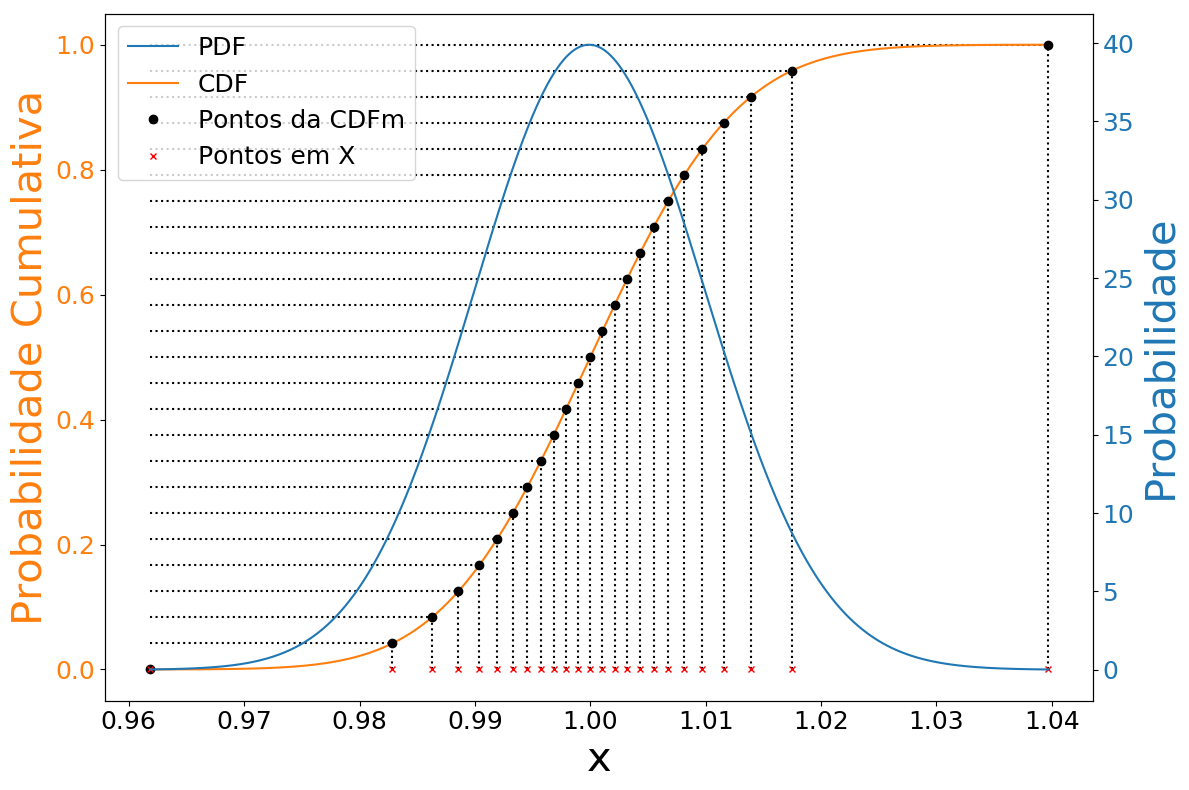
\includegraphics[width=\textwidth]{./figuras/CDFm_lognormal_001.png}
		\caption{}
		\label{fig:log001}
	\end{subfigure}
	\hfill
	\begin{subfigure}[b]{0.49\textwidth}
		\centering 
		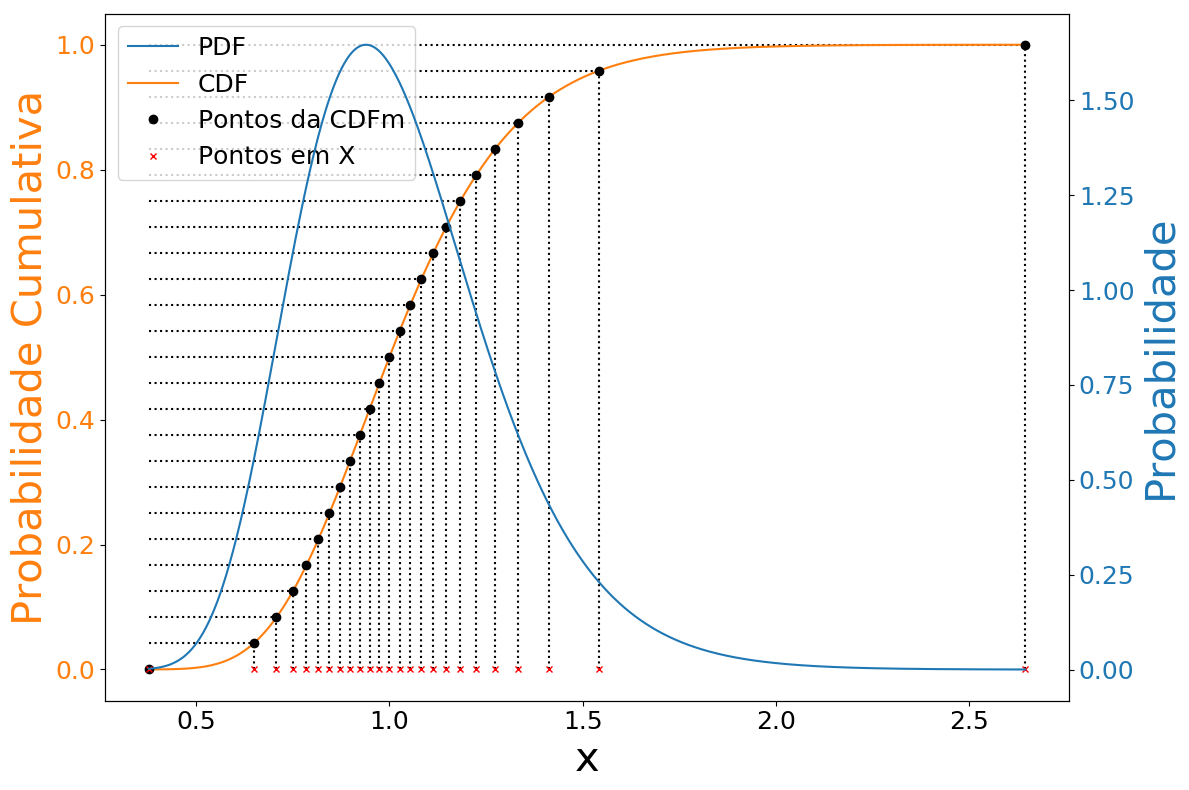
\includegraphics[width=\textwidth]{./figuras/CDFm_lognormal_025}
		\caption{}
		\label{fig:log025}
	\end{subfigure}
	
	\begin{subfigure}[b]{0.49\textwidth}
		\centering 
		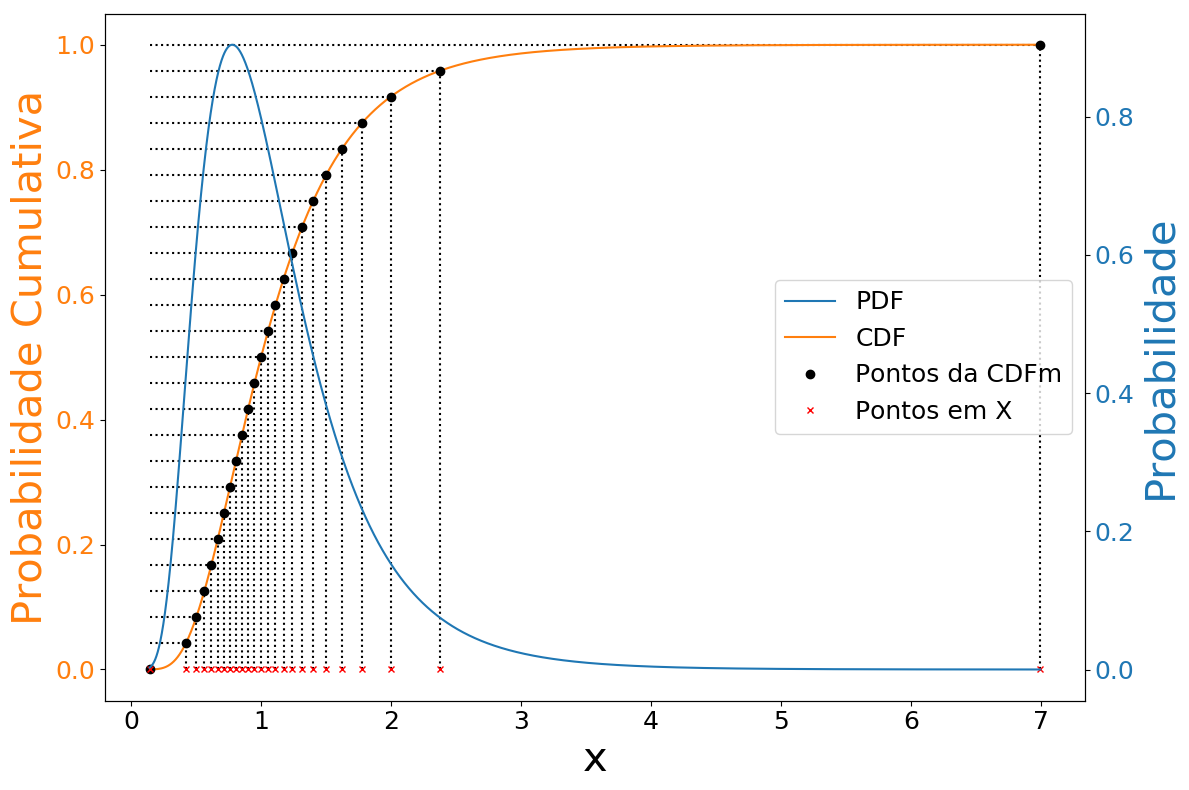
\includegraphics[width=\textwidth]{./figuras/CDFm_lognormal_05}
		\caption{}
		\label{fig:log050}
	\end{subfigure}
	\hfill
	\begin{subfigure}[b]{0.49\textwidth}
		\centering 
		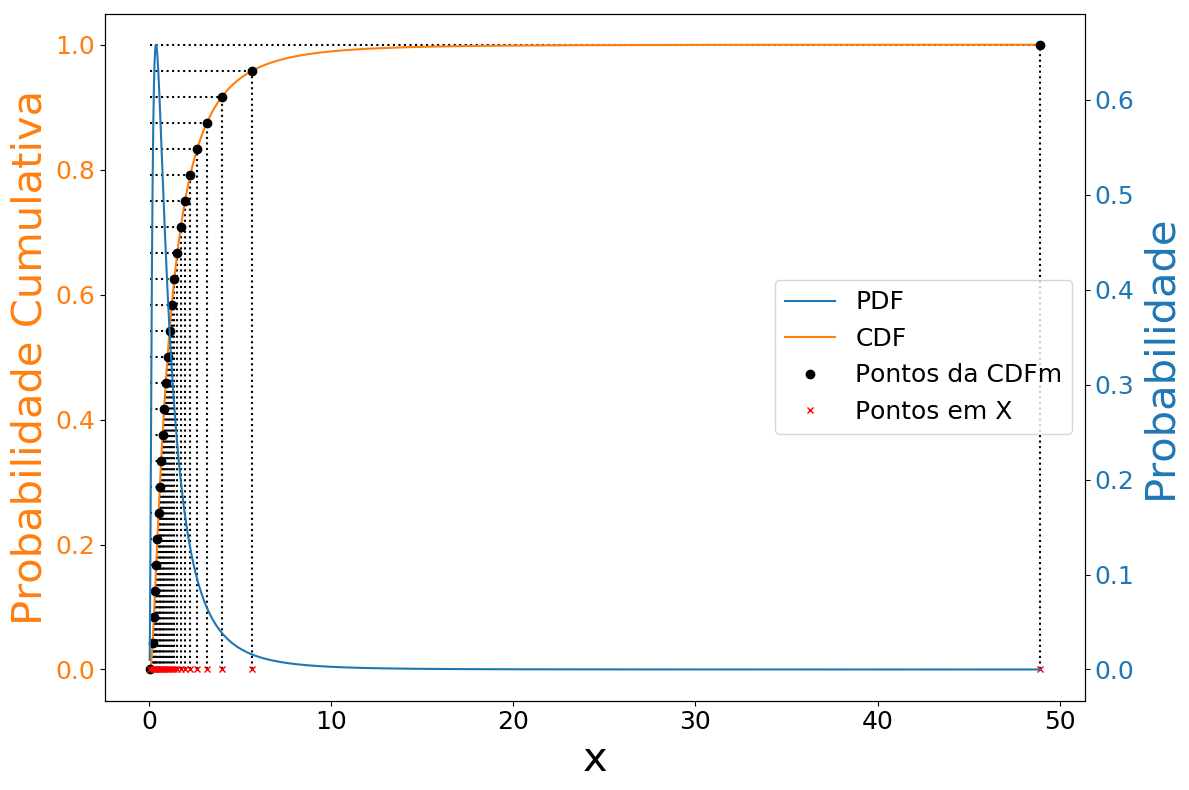
\includegraphics[width=\textwidth]{./figuras/CDFm_lognormal_1}
		\caption{}
		\label{fig:log100}
	\end{subfigure}
	
	\begin{subfigure}[b]{0.49\textwidth}
		\centering 
		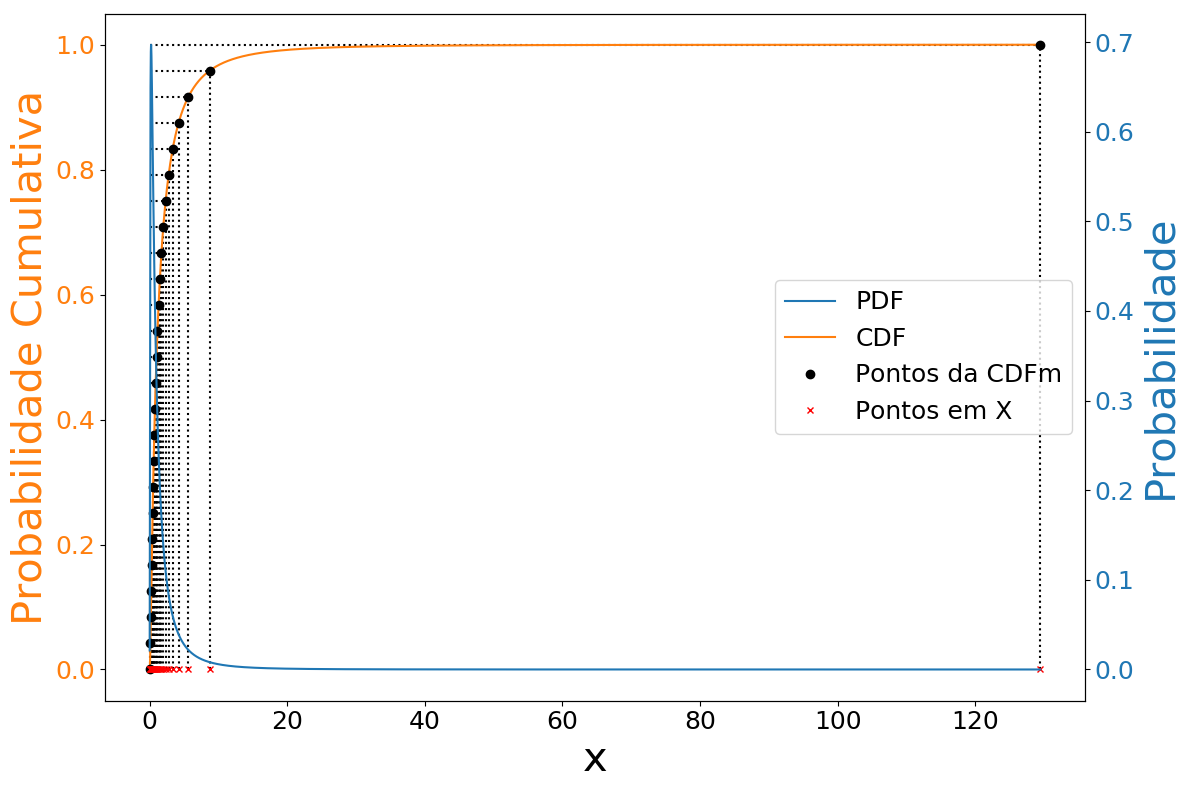
\includegraphics[width=\textwidth]{./figuras/CDFm_lognormal_125}
		\caption{}
		\label{fig:log125}
	\end{subfigure}
	\hfill
	\begin{subfigure}[b]{0.49\textwidth}
		\centering 
		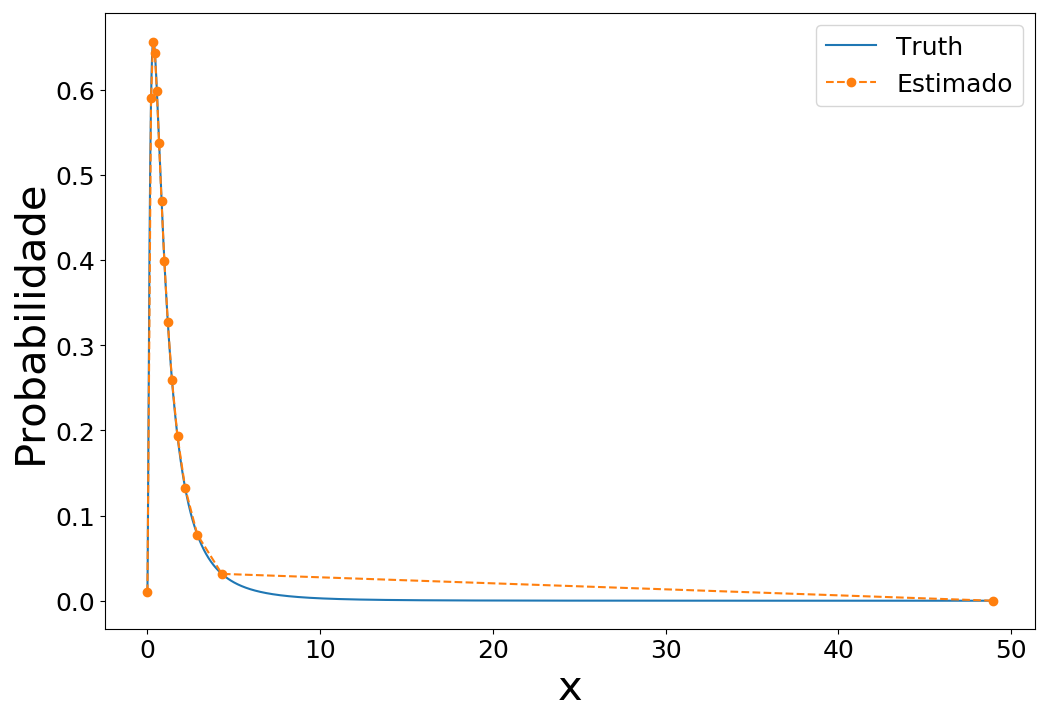
\includegraphics[width=\textwidth]{./figuras/CDFm_lognormal_15}
		\caption{}
		\label{fig:log150}
	\end{subfigure}
	\caption{Ilustração do método \textit{CDFm} aplicado à uma distribuição lognormal em que: (a) possui $\sigma = 0.01$; (b) possui $\sigma = 0.25$; (c) possui $\sigma = 0.5$; (d) possui $\sigma = 1$; (e) possui $\sigma = 1.25$; e (f) possui $\sigma = 1.5$}
	\label{fig:Lognormal_cdf}
\end{figure}

\begin{figure}[H]
	\centering
	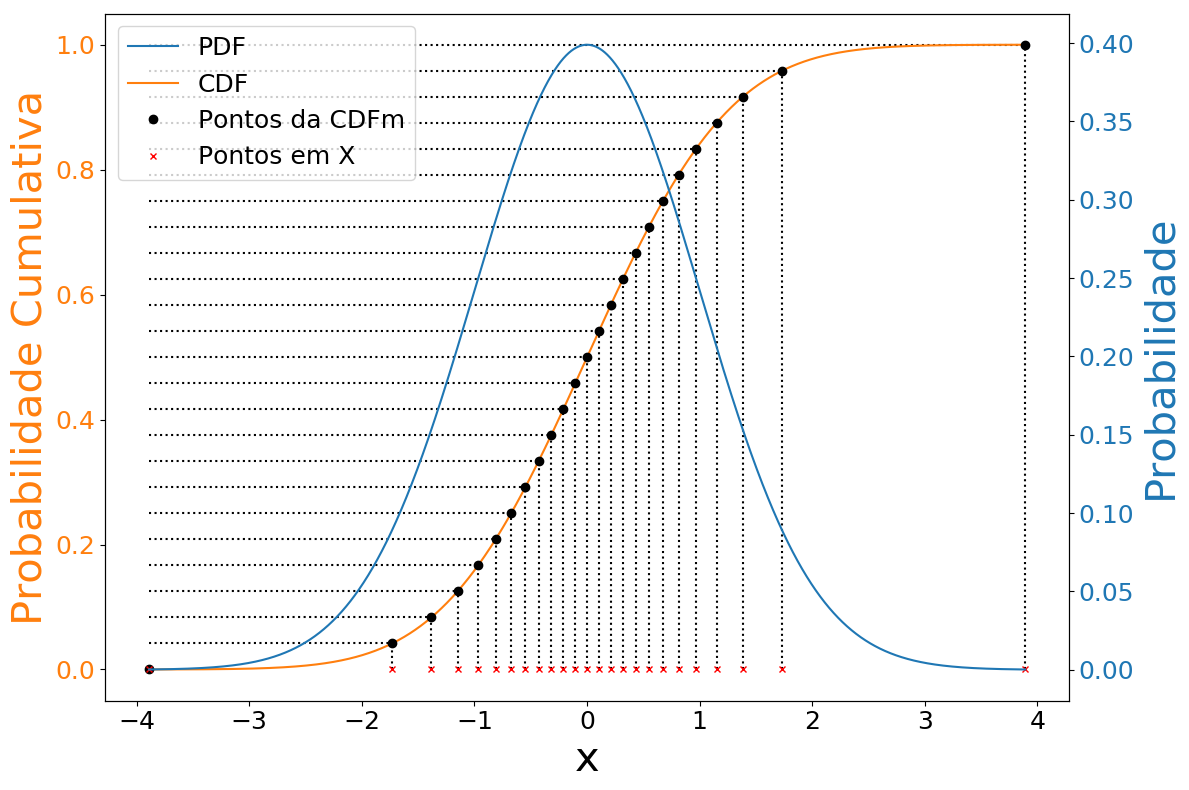
\includegraphics[width=0.6\linewidth]{./figuras/CDFm_normal_1}
	\caption{Ilustração da discretização da distribuição Gaussiana baseada em sua CDF.}
	\label{fig:CDFm_curve}
\end{figure}

\color{red} COLOCAR AQUI A FIGURA COM DATASET P/ CDFM \color{black}

Como este método baseia-se na \ac{CDF}, quando maior a variação na \ac{PDF}, mais rápido a CDF sobe, fazendo assim com que este método coloque mais pontos nas regiões de alta probabilidade e poucos pontos nas regiões de baixa probabilidade, sendo assim um método imune à \textit{outliers}.

\subsection{\textit{PDFm}}
Este método, denominado de \ac{PDFm} também usa a técnica de reflexão aplicada ao método da \textit{CDFm}, mas função de referência a própria \ac{PDF}, ao invés da sua \ac{CDF}. A Figura~\ref{fig:PDFm_curve} mostra como este método funciona para a distribuição Normal,a Figura~\ref{fig:Lognormal_pdf} para a distribuição Lognormal e a Figura~XXXX para dados gerados. Ela possui o efeito de incrementar o número de pontos onde a primeira derivada da \ac{PDF} é maior, ou seja, quanto maior a inclinação da curva, mais pontos são colocados.

\begin{figure}[H]
	\centering
	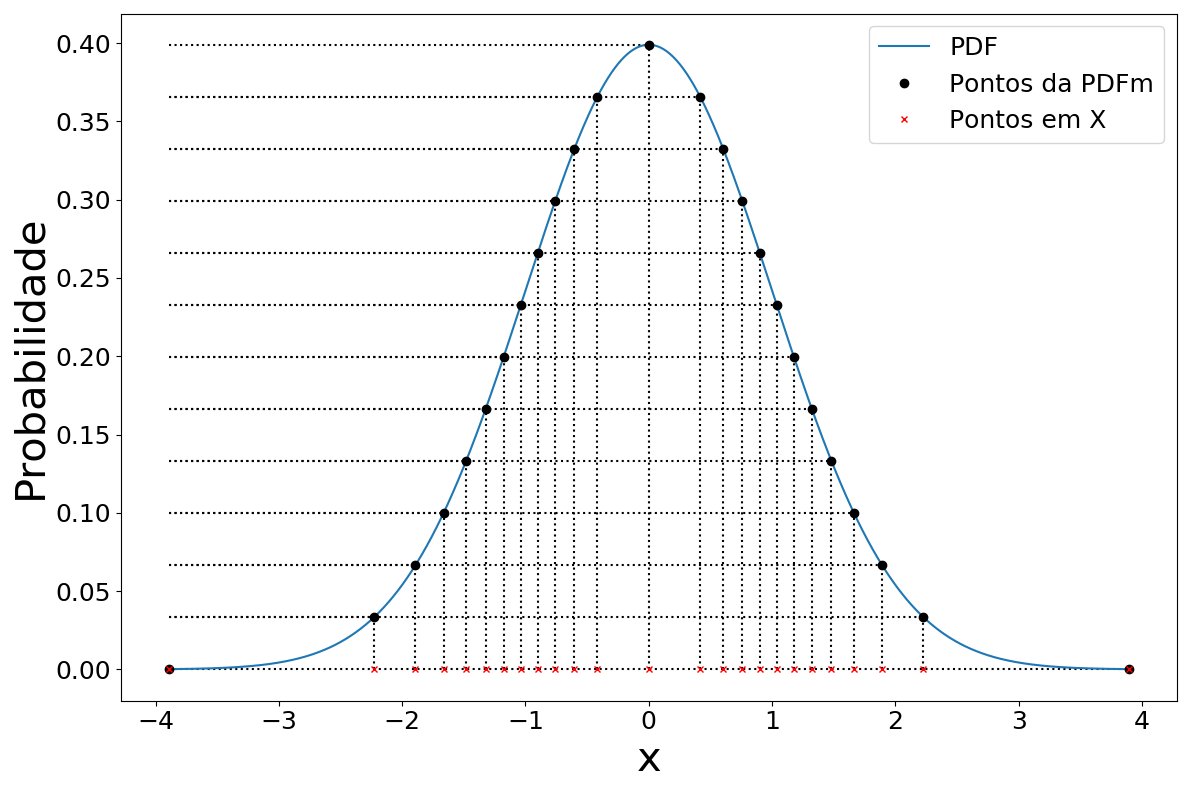
\includegraphics[width=0.67\linewidth]{./figuras/PDFm_normal_1}
	\caption{Ilustração da discretização da distribuição Gaussiana baseada em sua PDF.}
	\label{fig:PDFm_curve}
\end{figure}

{\color{red} COLOCAR GRÁFICO 2X3}

\begin{figure}[H]
	\centering
	\begin{subfigure}[b]{0.49\textwidth}
		\centering 
		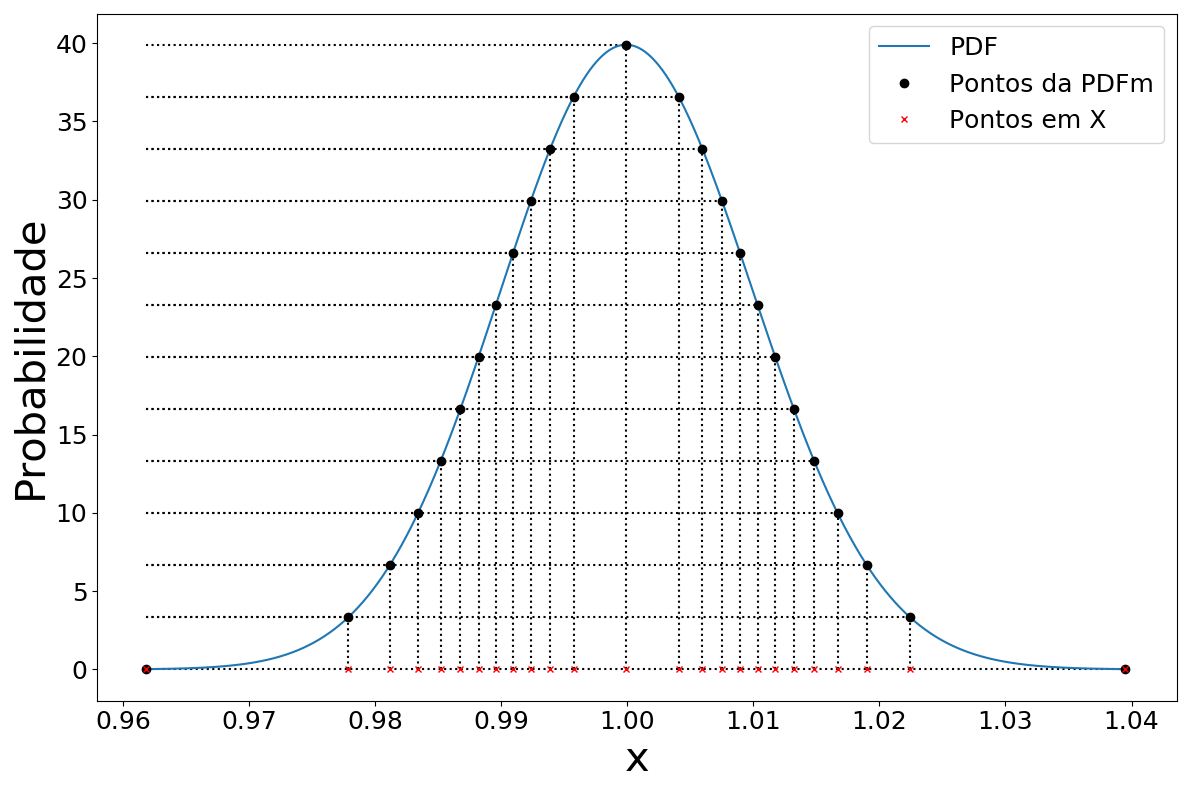
\includegraphics[width=\textwidth]{./figuras/PDFm_lognormal_001.png}
		\caption{}
		\label{fig:pdflog001}
	\end{subfigure}
	\hfill
	\begin{subfigure}[b]{0.49\textwidth}
		\centering 
		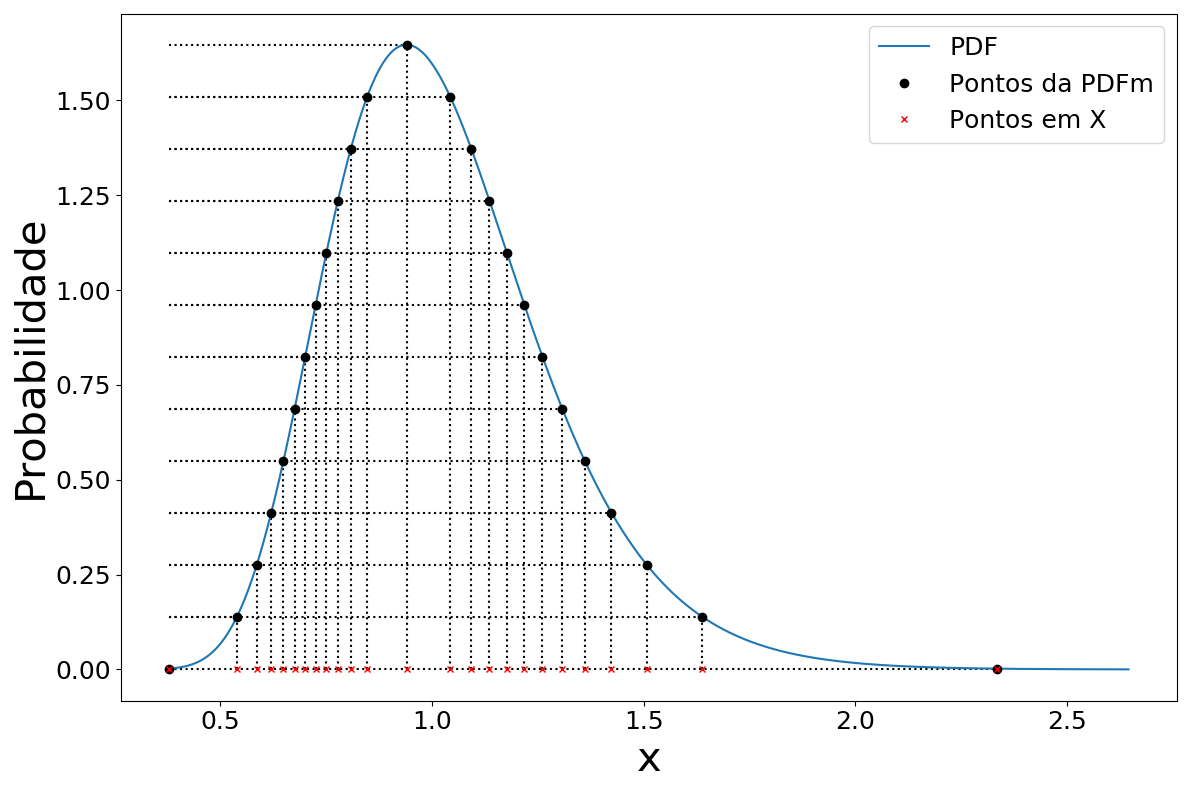
\includegraphics[width=\textwidth]{./figuras/PDFm_lognormal_025}
		\caption{}
		\label{fig:pdflog025}
	\end{subfigure}
	
	\begin{subfigure}[b]{0.49\textwidth}
		\centering 
		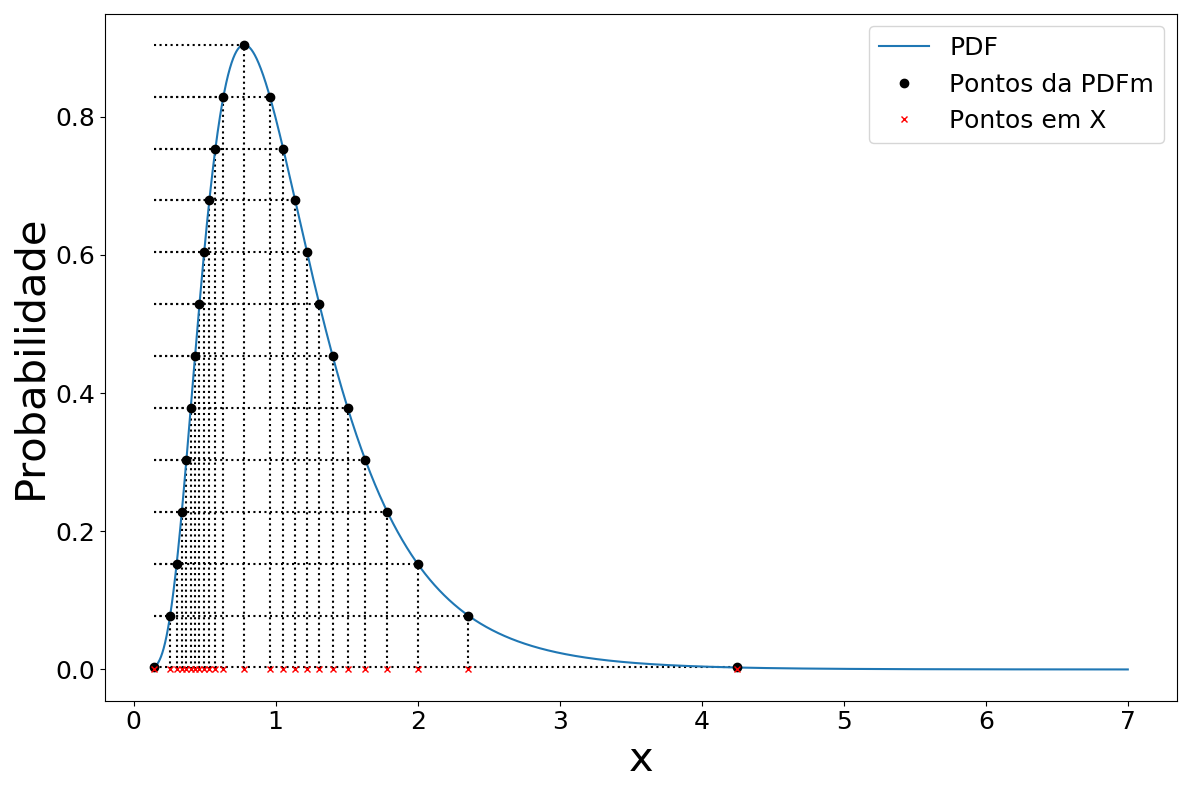
\includegraphics[width=\textwidth]{./figuras/PDFm_lognormal_05}
		\caption{}
		\label{fig:pdflog050}
	\end{subfigure}
	\hfill
	\begin{subfigure}[b]{0.49\textwidth}
		\centering 
		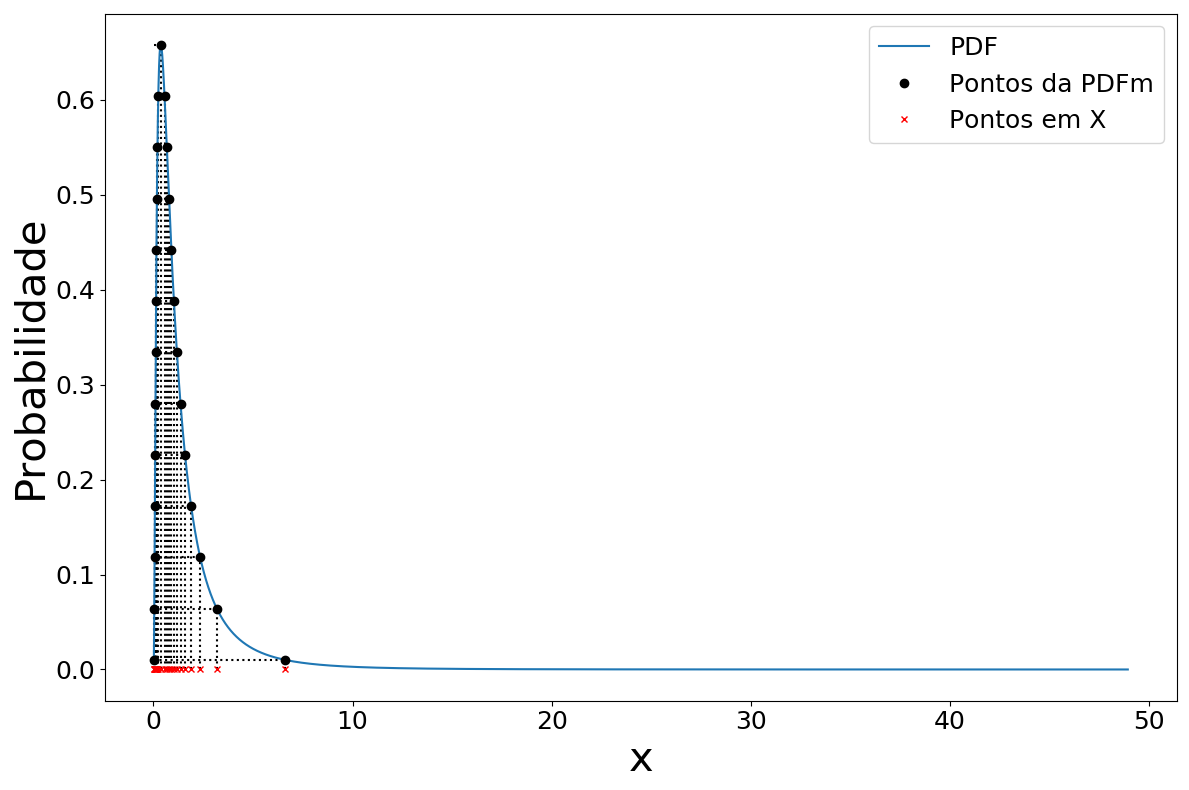
\includegraphics[width=\textwidth]{./figuras/PDFm_lognormal_1}
		\caption{}
		\label{fig:pdflog100}
	\end{subfigure}
	
	\begin{subfigure}[b]{0.49\textwidth}
		\centering 
		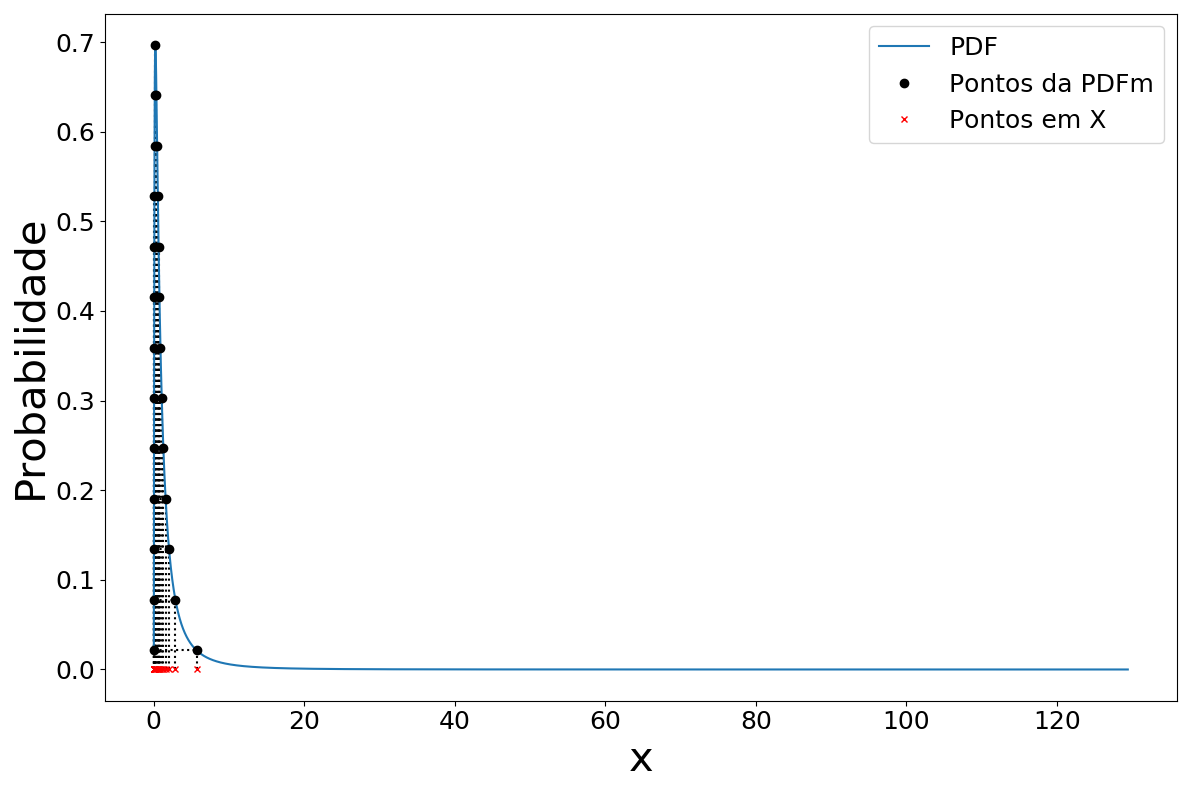
\includegraphics[width=\textwidth]{./figuras/PDFm_lognormal_125}
		\caption{}
		\label{fig:pdflog125}
	\end{subfigure}
	\hfill
	\begin{subfigure}[b]{0.49\textwidth}
		\centering 
		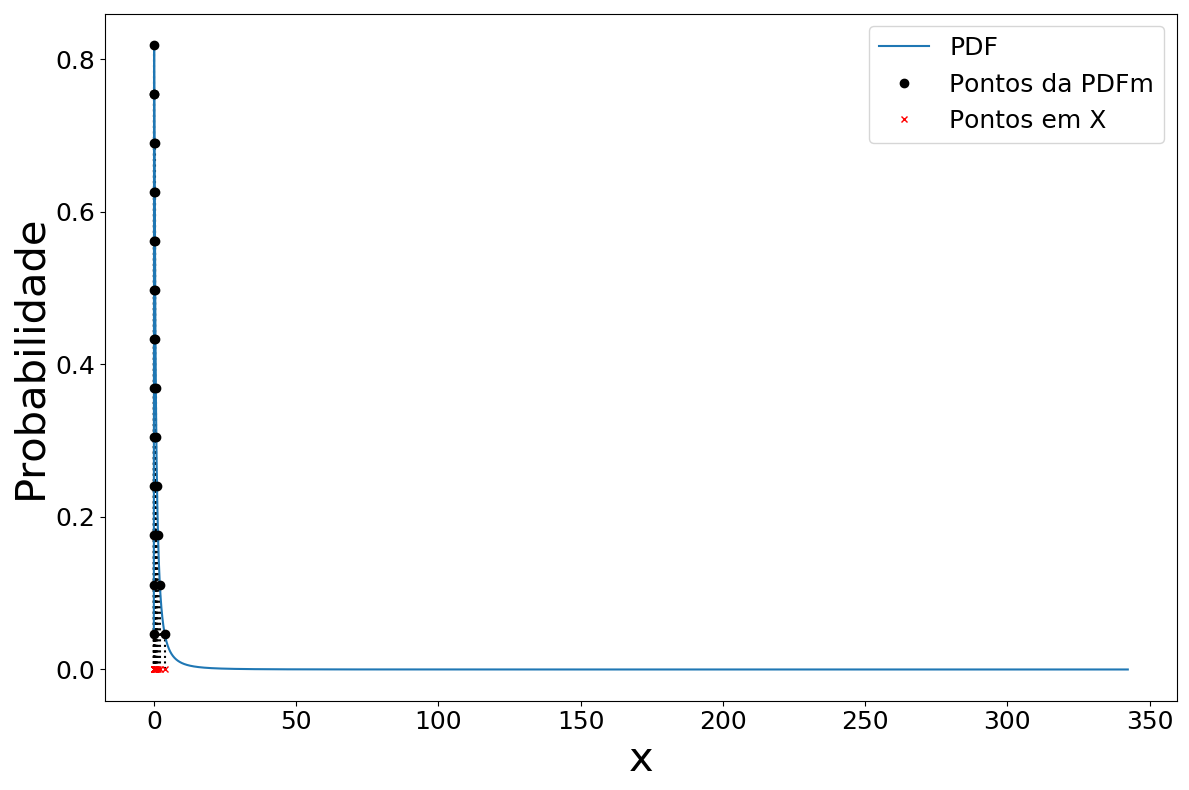
\includegraphics[width=\textwidth]{./figuras/PDFm_lognormal_15}
		\caption{}
		\label{fig:pdflog150}
	\end{subfigure}
	\caption{Ilustração do método \textit{PDFm} aplicado à uma distribuição Lognormal em que: (a) possui $\sigma = 0.01$; (b) possui $\sigma = 0.25$; (c) possui $\sigma = 0.5$; (d) possui $\sigma = 1$; (e) possui $\sigma = 1.25$; e (f) possui $\sigma = 1.5$}
	\label{fig:Lognormal_pdf}
\end{figure}

{\color{red} COLOCAR GRÁFICO DOS DATASETS}

\subsection{\textit{iPDF1}}

O método da \ac{iPDF1} reflete os valores verticais para o eixo horizontal usando a \ac{CDF} da primeira derivada da \ac{PDF} como uma transformação de base, como é ilustrado nas Figuras~\ref{fig:dPDF1} e \ref{fig:dPDF2}
{\color{red} COLOCAR O GRÁFICO DA DERIVADA EM ANEXO E AQUI O GRÁFICO DA CDF PARA A LOGNORMAL E COM OS DATASETS}
\begin{figure}[!ht]
	\centering
	\begin{subfigure}[b]{0.44\textwidth}
		\centering 
		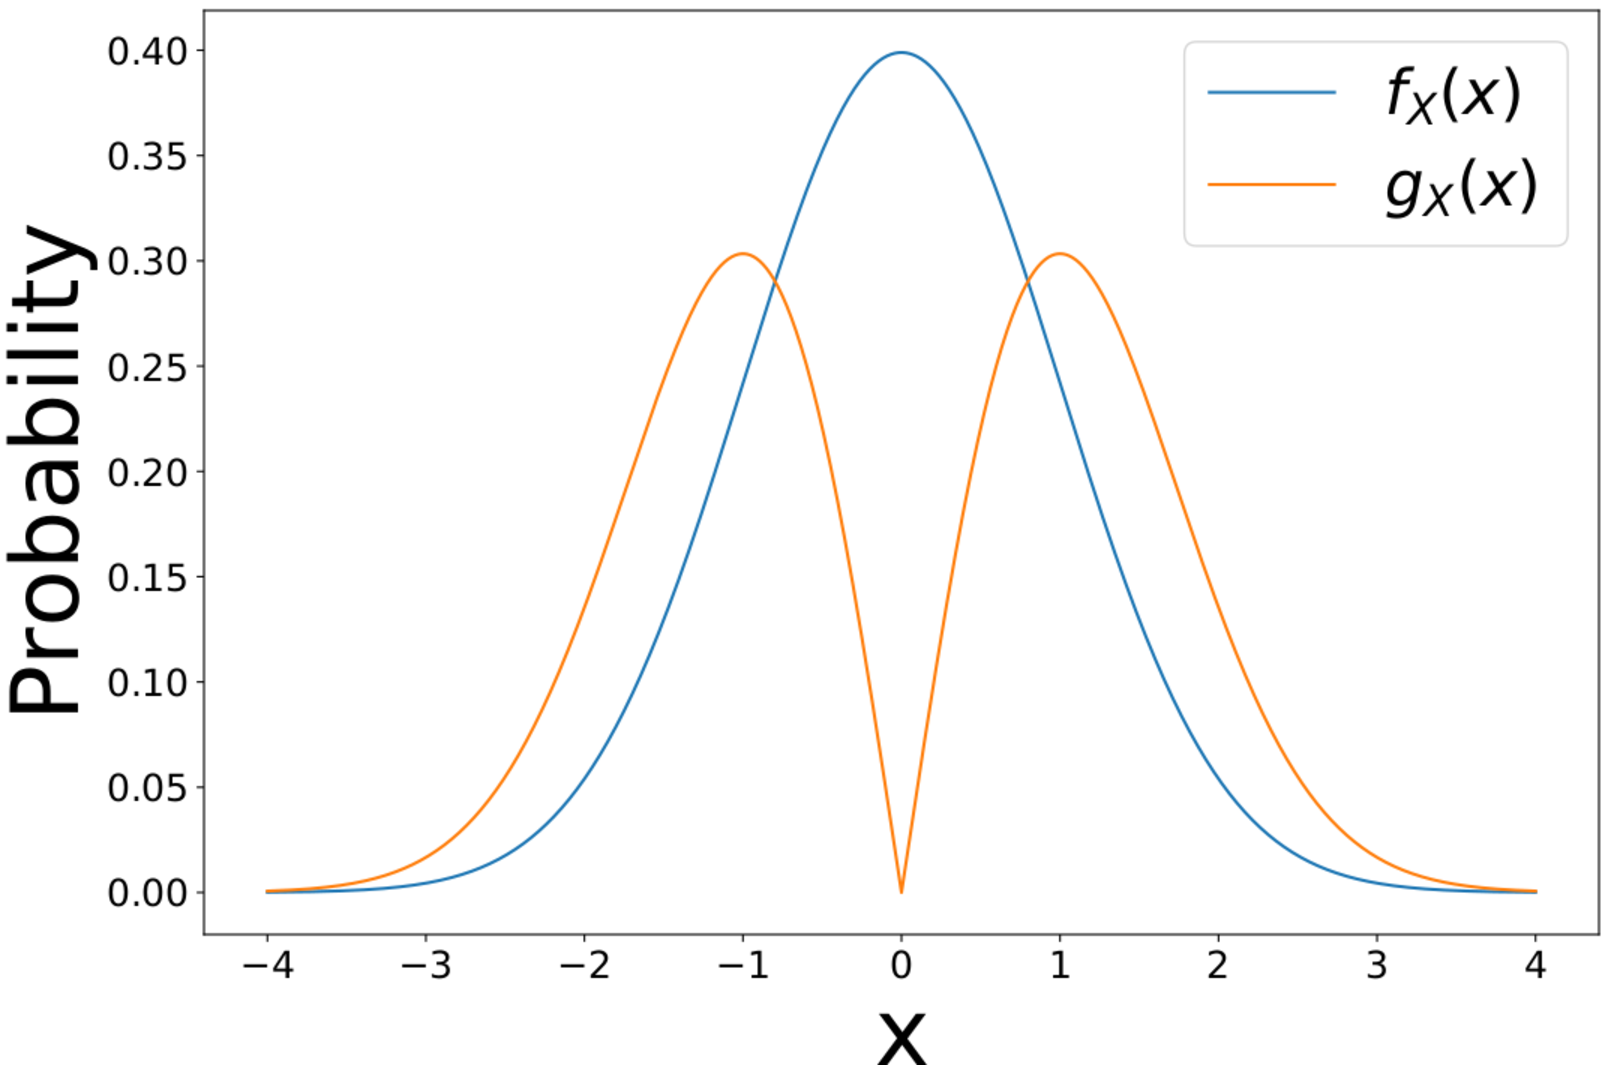
\includegraphics[width=\textwidth]{./figuras/dpdf1}
		\caption{}
		\label{fig:dPDF1}
	\end{subfigure}
	\hfill
	\begin{subfigure}[b]{0.47\textwidth}
		\centering 
		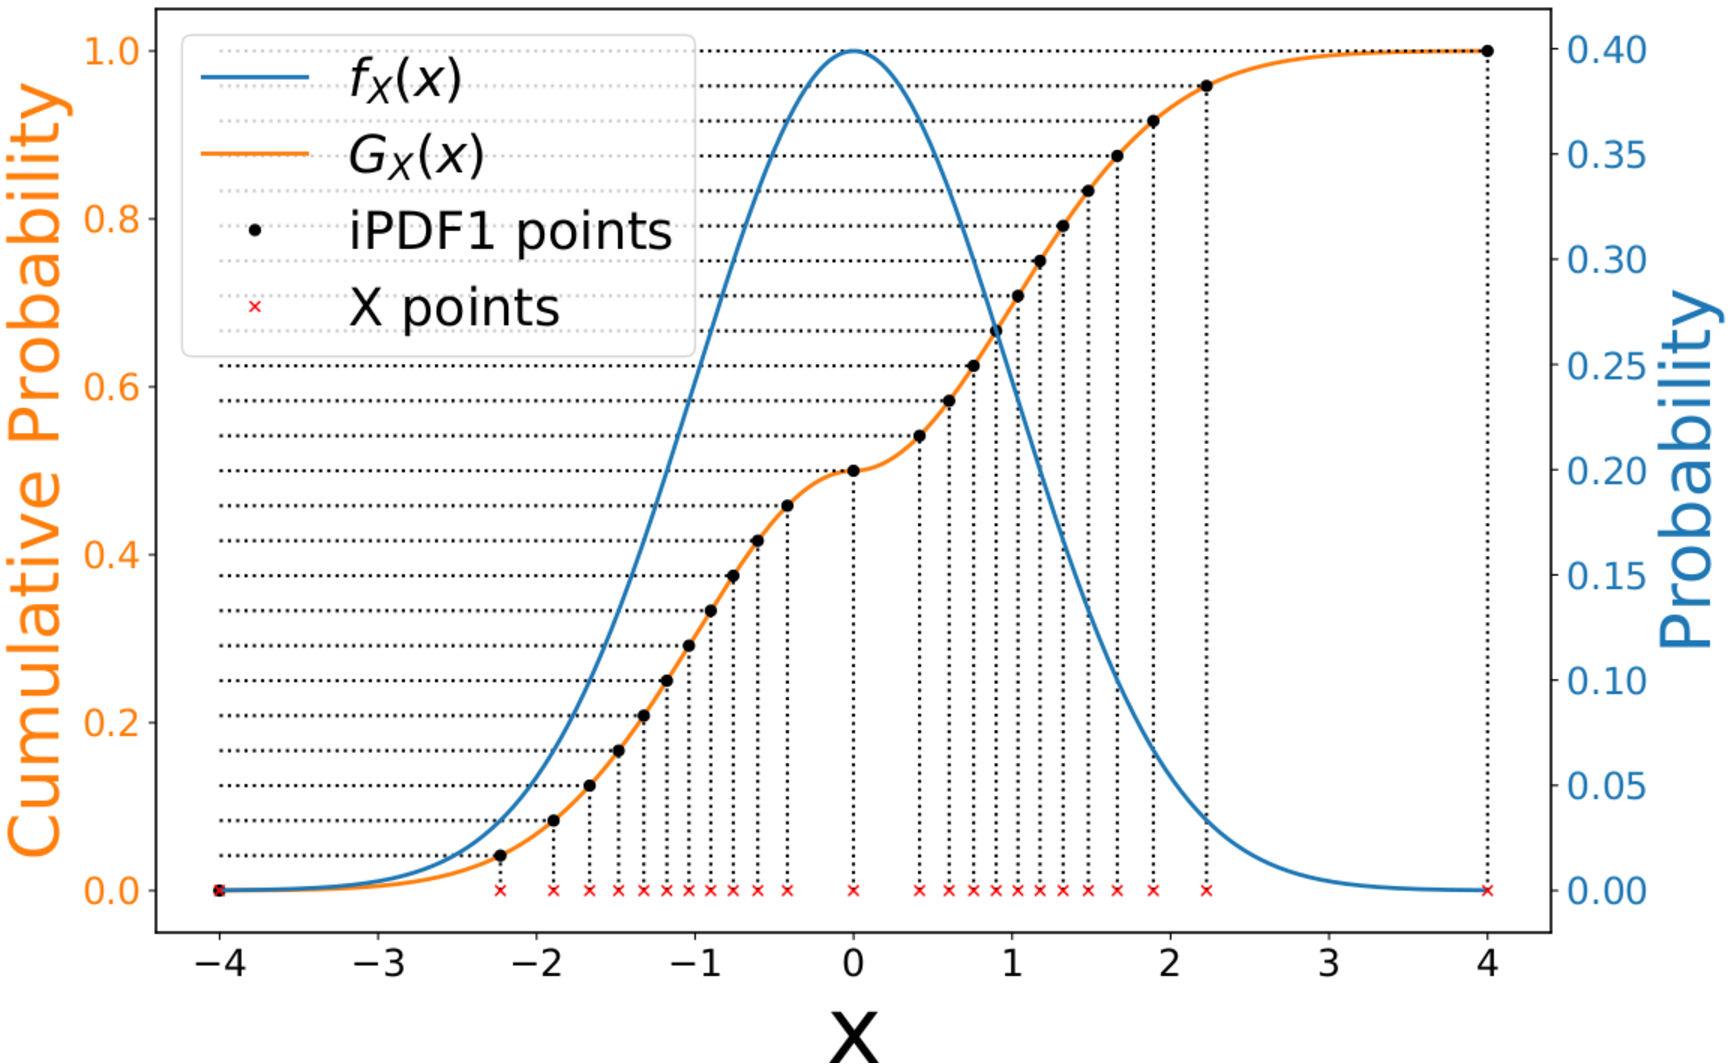
\includegraphics[width=\textwidth]{./figuras/dpdf2}
		\caption{}
		\label{fig:dPDF2}
	\end{subfigure}
\caption{PDF Gaussiana e sua primeira derivada à esquerda. Ilustração da discretização da distribuição Gaussiana baseada na CDF da sua primeira derivada à direita.}
\label{fig:dPDF}
\end{figure}

As equações \eqref{equ:dpdf1} e \eqref{equ:dcdf} descrevem este método matematicamente.

\color{red} COLOCAR AQUI TB A EQUAÇÃO PRA LOGNORMAL \color{black}
\begin{equation}
\begin{array}{l}
\vspace{0.3cm}\displaystyle \zeta(x) = \frac{|\mu-x|}{\sigma^3\sqrt{2\pi}}\cdot e^{\left(\frac{-(\mu-x)^2}{2\sigma^2}\right) } \\
\vspace{0.3cm} \displaystyle \int_{-\infty}^{\infty} \zeta(x)\cdot dx = c_1 \\
\displaystyle g_X(x) = \frac{\zeta(x)}{c_1}
\label{equ:dpdf1}
\end{array}
\end{equation}
onde $\zeta$ é a equação da distribuição da derivada da distribuição normal, $\mu$ é a média, $\sigma$ o desvio padrão, $x$ a variável aleatória, $c_1$ é a área abaixo da curva $\zeta$, e $g_X$ é a versão normalizada.	
A \ac{CDF} de $g_X$ ($G_X(x)$) é usada para transferir os valores da abscissa ao eixo da ordenada como mostra a  Figura~\ref{fig:dPDF2}.




Já para a aplicação com dados gerados, ilustrado na Figura~XXXX, precisamos utilizar a derivada discreta, que pode ser feita utilizando o método de diferenças finitas, que consiste em computar a inclinação de uma reta secante vizinha através dos pontos $(x,f(x))$ e $(x+h,f(x+h))$ \cite{burden2001numerical} que pode ser vista na Figura~XXXX. A inclinação dessa reta pode ser descrita pela Equação~\eqref{eq:derivdisc}

\begin{equation}
	{\displaystyle f'(x) = {f(x+h)-f(x) \over h}}
	\label{eq:derivdisc}
\end{equation}

onde \textit{h} é a distancia entre dois pontos vizinhos (\textit{bins}) e x o valor do \textit{bin}

{\color{red} BOTAR UMA FIGURA MANEIRA AQUI PRA EXPLICAR A DERIVADA DISCRETA}




\subsection{\textit{iPDF2}} \label{cap:ipdf2}
O método da \ac{iPDF2} é construído da mesma maneira da \textit{IPDF1} mas usando a segunda detivada ao invés da primeira, como é mostrado na Figura~\ref{fig:ddPDF1} e \ref{fig:ddPDF2}. Suas equações são mostradas em \eqref{equ:hx} e \eqref{equ:ddcdf}.

{\color{red} COLOCAR O GRÁFICO DA DERIVADA EM ANEXO E AQUI O GRÁFICO DA CDF PARA A LOGNORMAL E COM OS DATASETS}

\begin{figure}[ht]
	\centering
	\begin{subfigure}[b]{0.44\textwidth}
		\centering 
		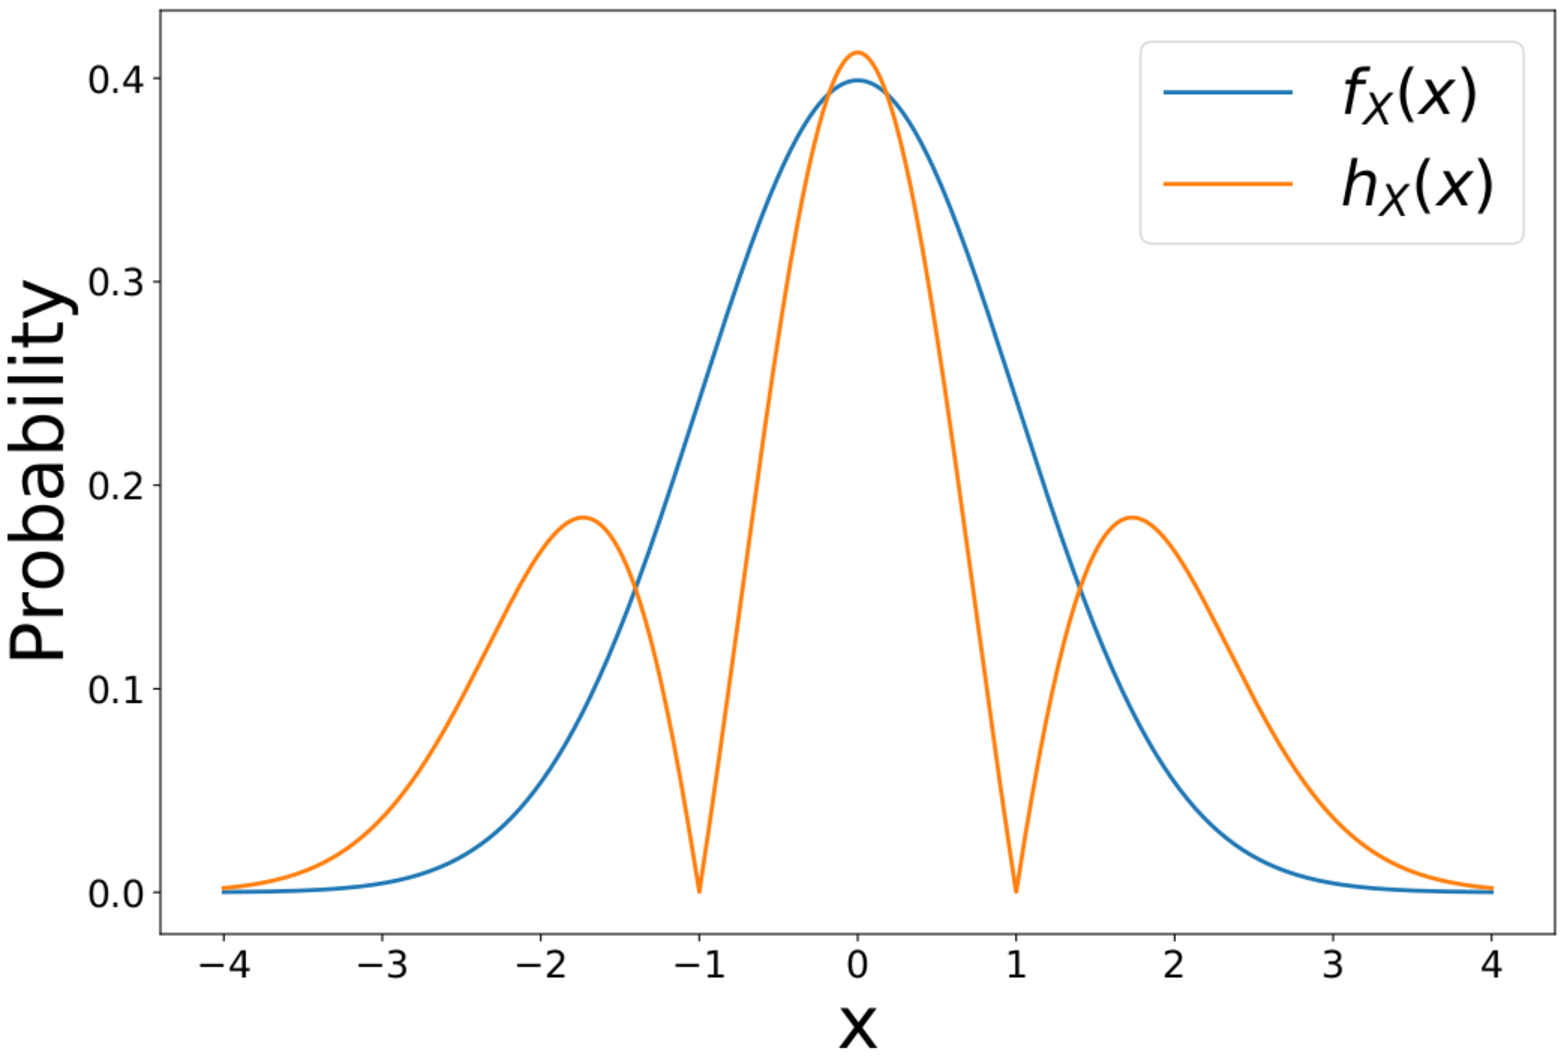
\includegraphics[width=\textwidth]{./figuras/ddpdf1.pdf}
		\caption{}
		\label{fig:ddPDF1}
	\end{subfigure}
	\hfill
	~ %add desired spacing between images, e. g. ~, \quad, \qquad, \hfill etc. 
	%(or a blank line to force the subfigure onto a new line)
	\begin{subfigure}[b]{0.47\textwidth}
		\centering 
		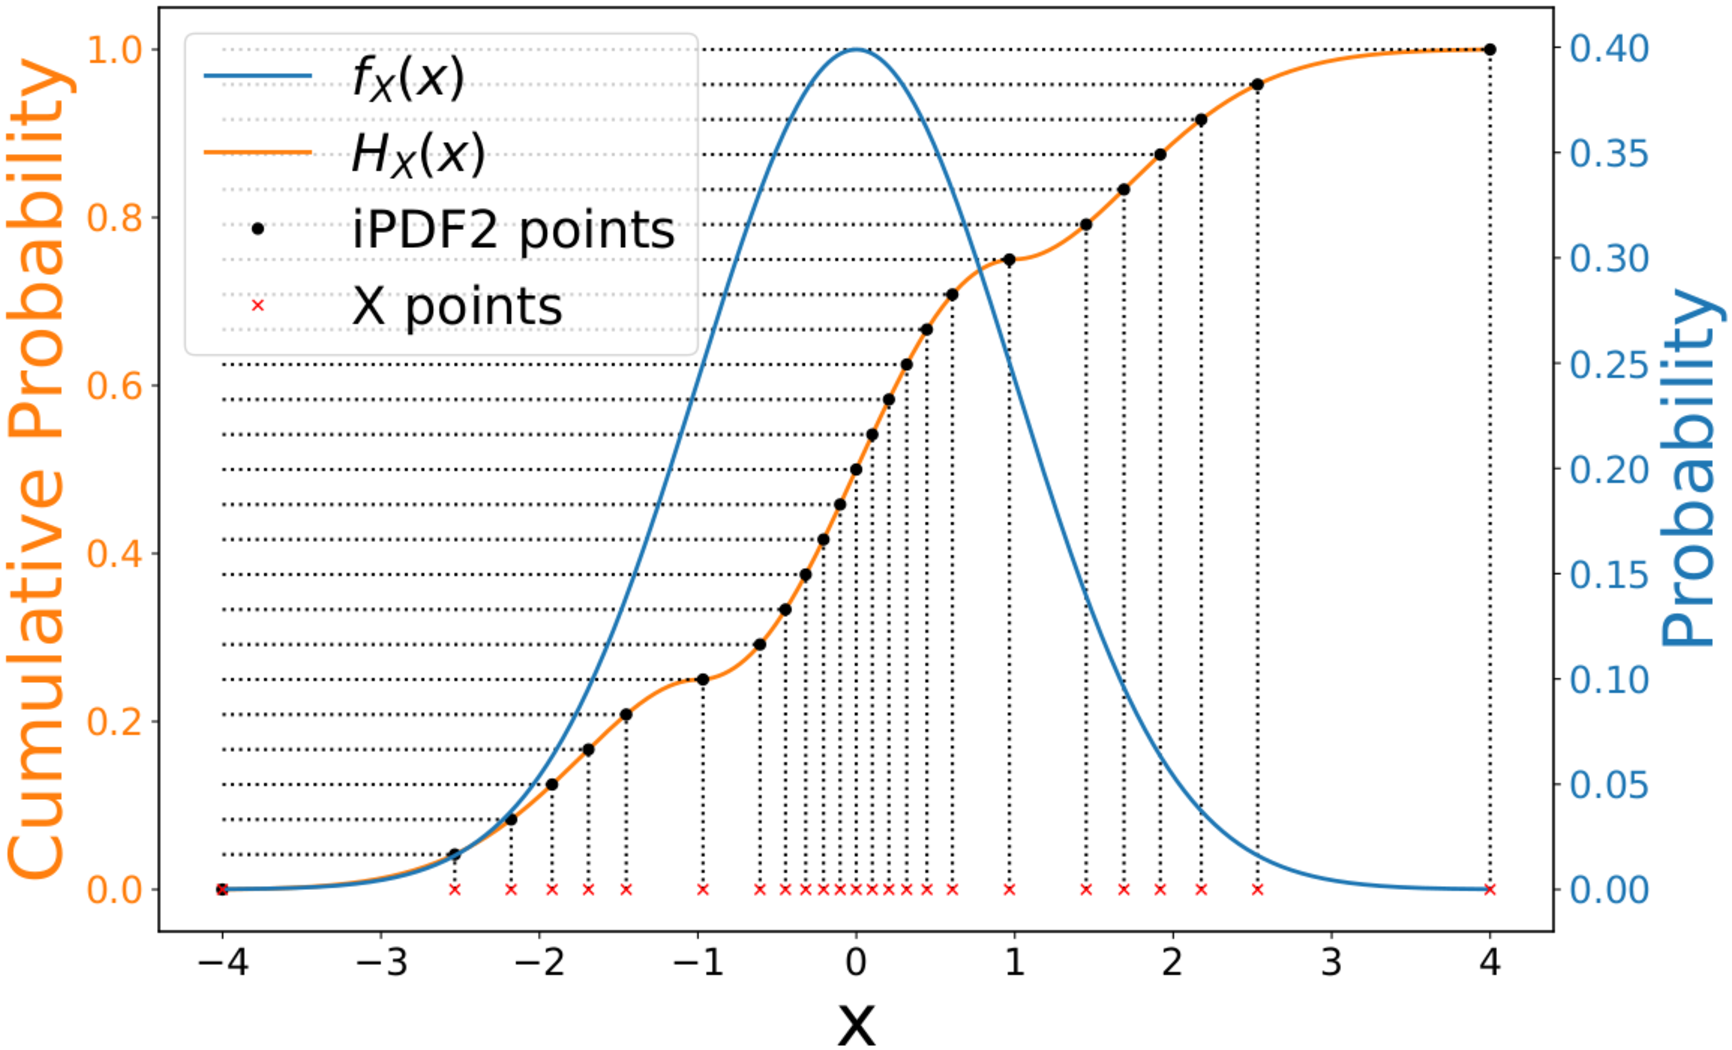
\includegraphics[width=\textwidth]{./figuras/ddpdf2.pdf}
		\caption{}
		\label{fig:ddPDF2}
	\end{subfigure}
	
	\caption{PDF Gaussiana e sua segunda derivada à esquerda. Ilustração da discretização da distribuição Gaussiana baseada na CDF da sua segunda derivada à direita.}
	\label{fig:ddPDF}
\end{figure}
\color{red} COLOCAR AQUI TB A EQUAÇÃO PRA LOGNORMAL \color{black}
\begin{equation}
\begin{array}{l}
\vspace{0.3cm}\displaystyle \eta(x) = \frac{|\sigma^2 - (\mu - x)^2|}{ \sigma^5\sqrt{2\pi}}\cdot e^{-\frac{(\mu - x)^2}{2 \sigma^2}} \\
\vspace{0.3cm} \displaystyle \int_{-\infty}^{\infty} \eta(x)\cdot dx = c_2 \\
\displaystyle h_X(x) = \frac{\eta(x)}{c_2}
\label{equ:hx}
\end{array}
\end{equation}
onde $\eta$ é a equação de distribuição de segunda derivada da distribuição Normal, $c_2$ é a área abaixo da curva desta distribuição, e $h_X$ é sua versão normalizada. 
Finalmente, $H_X(x)$ é a \ac{CDF} de $h_X$, dada por \eqref{equ:ddcdf}.

\begin{equation}
H_X(x) = \int_{-\infty}^x h_X(y)\cdot dy
\label{equ:ddcdf}
\end{equation}

Para os dados gerados, o precedimento é o mesmo descrito na Seção~\ref{cap:ipdf2} e a equação da segunda derivada discreta pode ser escrita pela Equação~\ref{eq:derivdisc2}.

\begin{equation}
{\displaystyle f''(x) = {f'(x+h)-f'(x) \over h}}
\label{eq:derivdisc2}
\end{equation}

\section{Ambiente de Análise}
Para analisar as diferenças entre a \ac{PDF} real e estimada ao longo de toda a extensão do eixo das abscissas, a área entre as duas \ac{PDF}s será usada como medida da estimação de erro. Além do mais, o eixo das abscissas foi dividida em $N$ regiões de mesmo tamanho, chamado \ac{RoI} \cite{ron1999art}. Essas regiões são compreendidas entre valores máximos e mínimos predefinidos do eixo horizontal. A Figura~XXXXX mostra este processo quando a abscissa é dividida em 20 regiões, todas compreendidas entre os valores $-4$ e $4$ do eixo $ x $.


{\color{red} COLOCAR AQUI O GRÁFICO COM O ERRO QUE TEM ZOOM}

A maneira que a \ac{RoI} é usada neste trabalho permitirá avaliar o erro de estimação em função de quatro diferentes parâmetros: Probabilidade; Eixo das abscissas; Primeira e Segunda Derivada. Para estimar os valores entre os pontos discretos, dois métodos de interpolação serão usados: interpolação pelo Vizinho Mais Próximo e Linear. 200 amostras serão usadas no processo de discretização. O erro de estimação tende a melhoras conforme o número de amostras aumenta mas sua característica geral não muda. Este último é a principal preocupação deste trabalho.

